\documentclass[11pt]{article}

\usepackage[margin=1in]{geometry}
\usepackage{amsmath,amssymb,amsthm}
\usepackage[T1]{fontenc}
\usepackage[utf8]{inputenc}
\usepackage{lmodern}
\usepackage{microtype}
\usepackage{booktabs}
\usepackage{longtable}
\usepackage[hidelinks]{hyperref}
\usepackage{parskip}
\usepackage{tikz}
\usetikzlibrary{positioning}

% No section numbering in subsection references but keep numbering
\setcounter{secnumdepth}{3}

\title{The Logical Geography of Mathematical Physics:\\
Constructive Calibration from Density Matrices\\to the Choice Axis\\[1em]
\large A Companion to the Constructive Calibration Programme (Paper~10, v5.0)}
\author{Paul Chun-Kit Lee\\New York University}
\date{February 2026}

\begin{document}
\maketitle

\begin{abstract}
This paper synthesizes the machine-verified results of the author's constructive calibration programme --- spanning functional analysis (Papers~2, 7), quantum spectra (Paper~4), general relativity (Papers~5, 13), uncertainty relations (Paper~6), statistical mechanics (Papers~8, 9, 20), quantum information (Paper~11), quantum decoherence (Paper~14), conservation laws (Paper~15), quantum measurement statistics (Paper~16), quantum gravity (Paper~17), particle physics (Paper~18), semiclassical quantum mechanics (Paper~19), quantum foundations (Papers~21, 24), radioactive decay (Paper~22), ergodic theory (Paper~25), classical mechanics (Paper~28), and subadditive sequence convergence (Paper~29) --- into a single interpretive framework. It contains no new theorems or formalizations. Its purpose is to assemble the calibration table, establish the certification methodology, formulate a working hypothesis, and pose a research program.

The calibration table now contains approximately forty-eight entries spanning BISH to undecidable, populated by machine-verified Lean~4 formalizations totalling approximately 21,249 lines of code across eleven domains of mathematical physics. The results establish that preparation uncertainty, finite-size approximations, quantum entanglement structure (Tsirelson bound, Bell state entropy, partial trace), CHSH violation (negation form), Kochen-Specker uncolorability, WKB transmission amplitudes, Schwarzschild interior finite-time physics, Bekenstein-Hawking algebraic correction, finite-step decoherence bounds, local conservation laws, Born probabilities, discrete Euler-Lagrange equations, and fermion mass ratios$^\ddagger$ are fully constructive (BISH); that measurement uncertainty, locale spatiality, and the strong law of large numbers require Dependent Choice (DC$_\omega$); that the mean ergodic theorem is equivalent to Countable Choice (CC) and Birkhoff's pointwise ergodic theorem is equivalent to the stronger Dependent Choice (DC), separating ensemble convergence from individual-trajectory convergence along a refined choice axis AC$_0 < $ CC $ < $ DC (Paper~25); that WKB turning-point decisions, Bell's disjunctive conclusion, and Kochen-Specker sign decisions require exactly LLPO; that exact spectral membership and radioactive decay (eventual detection from non-zero decay rate) require Markov's Principle (MP); that singular states, the bidual gap, and phase classification (magnetization zero-test) require WLPO; that the thermodynamic limit, geodesic incompleteness, Bekenstein-Hawking entropy density convergence, exact decoherence, and global energy existence require exactly LPO; Paper~29 identifies the generic mechanism as Fekete's Subadditive Lemma, which is equivalent to LPO over BISH, with BMC as the proof-theoretic vehicle; and that compact optimization (the extreme value theorem on $[a,b]$) and action minimizer existence in classical mechanics require the Fan Theorem (FT), on a branch independent of the omniscience chain.

The logical geography is a partial order with three independent branches and a refined choice axis: the omniscience spine (BISH $<$ LLPO $<$ WLPO $<$ LPO), the choice hierarchy (CC $<$ DC, with CC calibrated via the mean ergodic theorem and DC via Birkhoff's theorem), Markov's Principle (orthogonal to the spine), and the Fan Theorem (independent of all of the above). CRM detects a structural identity invisible to informal analysis: Bell nonlocality and Kochen-Specker contextuality --- physically distinct phenomena --- share the identical logical cost (LLPO). Observable-dependent logical cost is established: the same physical system (1D Ising model) requires BISH, WLPO, LPO, or FT depending on the observable queried. The same Fekete~$\equiv$~LPO equivalence (Paper~29, with BMC as the extraction mechanism) now governs completed limits in five independent domains --- statistical mechanics, general relativity, quantum decoherence, conservation laws, and quantum gravity --- a domain invariance that substantially strengthens the evidence that the costs are intrinsic to the physics.

We establish a certification methodology with three levels --- mechanically certified, structurally verified, and intentional classical content --- that addresses the relationship between Lean~4's classical metatheory (Mathlib) and the series' constructive claims. We formulate a working hypothesis: all non-constructive costs arise from infinite-dimensional idealization layers, not from finite-dimensional or finite-time physical content. We present formulation-invariance evidence (Papers~8, 9), formulation-stratification evidence (Paper~28: Newtonian equations are BISH, Lagrangian variational principles cost FT), domain-invariance evidence (Papers~8, 13, 14, 15, 17), observable-dependent cost evidence (Paper~20), and structural identity evidence (Papers~21, 24), and situate the proposal within the broader landscape of constructive approaches to physics.

\noindent$^\ddagger$Paper~18 is a numerical (Python) computation, not a Lean~4 formalization.
\end{abstract}

\section{Executive Summary: The Programme at a Glance}

The following summarizes every paper in the series, what it proves, and why it matters for the programme.

\textbf{Paper~2} (Bidual gap / WLPO). Physicists routinely identify a Hilbert space with its double dual when writing bra-ket notation. This identification requires WLPO --- the ability to decide ``all entries are zero'' vs.\ ``not all are zero'' for an infinite sequence. The gap between a Banach space and its bidual is exactly the gap between constructive and non-constructive mathematics. \emph{Calibration:} bidual-gap witness $\equiv$ WLPO.

\textbf{Paper~4} (Quantum spectra / AxCal). Five spectral properties of self-adjoint operators --- from approximate eigenvalues to exact spectral membership --- require five different logical principles, spanning BISH to WLPO with MP on an orthogonal axis. The entire edifice of quantum mechanics rests on spectral theory; this is its logical price list.

\textbf{Paper~5} (Schwarzschild curvature / BISH). The curvature tensor of the Schwarzschild solution at any finite radius is fully constructive. General relativity's local content is constructively innocent; non-constructive cost enters only through global extension.

\textbf{Paper~6} (Heisenberg uncertainty / BISH). The Robertson-Schr\"odinger uncertainty inequality is BISH --- pure Cauchy-Schwarz geometry in finite-dimensional inner product spaces. One of quantum mechanics' most philosophically loaded results requires no non-constructive logic whatsoever.

\textbf{Paper~7} (Trace-class bidual / WLPO). Extends Paper~2 to the physically relevant setting of trace-class and density operators. Confirms the WLPO cost is not an abstraction artifact.

\textbf{Paper~8} (1D Ising / LPO). The programme's cleanest demonstration. Finite Ising model is BISH. Thermodynamic limit costs exactly LPO. Both directions proved, equivalence tight. The non-constructive content enters through the infinite-volume limit, not through the physics.

\textbf{Paper~9} (Ising formulation-invariance). Transfer matrix and partition function formulations yield identical logical cost. The cost is intrinsic to the physics, not the formalism.

\textbf{Paper~11} (Entanglement / BISH). Tsirelson's bound $2\sqrt{2}$ is BISH. The compositional tensor product structure is where non-constructive content enters, not the correlations themselves.

\textbf{Paper~13} (Event horizon / LPO). The event horizon coincides with the logical boundary --- the point where constructive mathematics can no longer describe the geometry. The most natural boundary in GR coincides with the most natural boundary in constructive logic.

\textbf{Paper~14} (Decoherence / LPO). Decoherence in the infinite-environment limit costs LPO. Confirms the BMC~$\equiv$~LPO pattern in a third domain.

\textbf{Paper~15} (Noether / BISH+LPO). Conservation laws from continuous symmetries are BISH in finite dimensions. Global energy existence costs LPO. The sign of the conserved density is logically significant.

\textbf{Paper~16} (Born rule / DC$_\omega$). The measurement problem's probabilistic infrastructure is BISH; the controversy lives in the infinite limit. Every finite collection of outcomes is BISH; exact frequentist convergence requires DC$_\omega$.

\textbf{Paper~17} (Bekenstein-Hawking / LPO). Extends the programme to quantum gravity. The BH area-entropy formula's algebraic correction is BISH; entropy density convergence in the loop quantum gravity sum costs LPO via BMC. The fifth BMC~$\equiv$~LPO domain.

\textbf{Paper~18} (Fermion mass / BISH). A negative result that is methodologically essential. The Scaffolding Principle --- removing non-constructive scaffolding to reveal new physics --- produces nothing new for the fermion mass hierarchy. The idle machinery is idle. (Numerical Python computation.)

\textbf{Paper~19} (WKB tunneling / LLPO). First physical LLPO calibration. Three tiers: specific transmission amplitudes (BISH), turning-point existence (LLPO via IVT), semiclassical limit (LPO). Quantum mechanics itself is BISH; the non-constructive cost lies in classical geometry.

\textbf{Paper~20} (Observable-dependent cost / WLPO). The same 1D Ising model requires different logical principles for different observables --- free energy convergence (LPO), phase classification via magnetization zero-test (WLPO), finite bounds (BISH), parameter-space optimization (FT). Logical cost is not a property of the system but of the question asked.

\textbf{Paper~21} (Bell nonlocality / LLPO). The step from ``local realism is refuted'' (BISH, via CHSH violation) to ``either locality or realism fails'' (the disjunctive conclusion) costs exactly LLPO. The precise logical cost of disjunction without witness.

\textbf{Paper~22} (Markov decay / MP). ``If a nucleus has a non-zero decay rate, it will eventually be detected as having decayed'' requires Markov's Principle. The tunneling traversal time controversy is diagnosed as a disagreement about MP, not about physics.

\textbf{Paper~23} (Fan Theorem / FT). Compact optimization (the extreme value theorem on $[a,b]$) requires the Fan Theorem, independent of the entire omniscience chain. Different physical reasoning (completed limits vs.\ compactness arguments) draws on different logical wells. The hierarchy is a tree, not a ladder. Zero custom axioms.

\textbf{Paper~24} (Kochen-Specker / LLPO). KS contextuality has the same logical cost as Bell nonlocality (LLPO). CRM detects a hidden structural identity: two physically unrelated no-go theorems --- one involving spatially separated systems, the other a single system --- are the same logical phenomenon (``disjunction without constructive witness'') in different physical clothing.

\textbf{Paper~25} (Choice axis / CC / DC). Opens a second axis in the calibration: the choice hierarchy AC$_0 < $ CC $ < $ DC. The mean ergodic theorem (von Neumann, 1932) is equivalent to Countable Choice (CC); Birkhoff's pointwise ergodic theorem is equivalent to Dependent Choice (DC). The weak law of large numbers calibrates to CC; the strong law to DC. Ensemble-level convergence (L$^2$ averages) requires CC; individual-trajectory convergence (pointwise a.e.) requires DC. The Type-level reverse direction is non-trivially formalized (395 lines). \emph{Calibration:} Mean Ergodic $\equiv$ CC; Birkhoff $\equiv$ DC.

\textbf{Paper~28} (Newton vs.\ Lagrange / BISH+FT). Classical mechanics' two formulations are constructively inequivalent. The Newtonian formulation (solving the Euler-Lagrange equation) is BISH --- an explicit algebraic solution. The Lagrangian formulation (asserting the action functional attains its minimum) requires the Fan Theorem. The variational interpretation is logically dispensable; the equations are the physical content. \emph{Calibration:} discrete EL equations = BISH; action minimizer existence $\equiv$ FT.

\textbf{Paper~29} (Fekete's lemma / LPO). The generic mechanism underlying the five-domain LPO pattern. Fekete's Subadditive Lemma --- every subadditive sequence with $u_n/n$ bounded below converges --- is equivalent to LPO over BISH. Since the thermodynamic limit proceeds via subadditivity of the log-partition function, LPO is the ineliminable cost of the generic route. Exactly solvable models (Papers~8, 9) and cluster expansions bypass Fekete at BISH cost. Resolves Problem~1. \emph{Calibration:} Fekete convergence $\equiv$ LPO.

\textbf{Paper~10} (this paper). Technical synthesis. Assembles the calibration table, establishes certification methodology, formulates the working hypothesis, and poses the research programme.

\textbf{Paper~12}. Historical companion. Traces the 150-year history of non-constructive commitments in mathematical physics from Cauchy through Cantor to the present, and argues that the constructive hierarchy tracks the physicist's layers of idealization.

\section{Introduction}

Mathematical physics is written in the language of classical mathematics. Physicists invoke the law of excluded middle, the axiom of choice, and the full strength of Zermelo-Fraenkel set theory without hesitation, and the resulting formalism produces spectacularly accurate predictions. The question of whether this logical strength is \emph{necessary} --- whether the same physical content could be extracted from weaker principles --- has been raised periodically since Brouwer, but has remained largely a philosophical curiosity. The practical success of classical mathematics leaves little incentive to investigate constructive alternatives.

This paper argues that the question deserves revival, and that recent machine-verified results in constructive reverse mathematics provide the tools to address it with unprecedented precision. The central observation is simple: when one examines the standard mathematical infrastructure of mathematical physics through a constructive lens, the logical principles required at each level of idealization fall into a structured hierarchy --- a partial order with three independent branches --- that correlates with the degree of physical abstraction.

\textbf{Scope and status.} This paper contains no new proofs or formalizations. All formal results are machine-verified in the twenty-two companion papers [Lee 2026a--2026w]. Our contribution here is interpretive: we assemble the verified results into a calibration table mapping layers of mathematical physics to positions in the constructive hierarchy, formulate a working hypothesis about what this mapping means, establish the series-wide certification methodology, and report the outcome of formulation-invariance, domain-invariance, observable-dependent cost, and structural identity tests. Papers~2, 5, 6, 7, 8, 9, 11, 13, 14, 15, 16, 17, 19, 20, 21, 22, 23, 24, 25, 28, and~29 employ constructive reverse mathematics (CRM) over Mathlib-based Lean~4 formalizations; Paper~4 employs the Axiom Calibration (AxCal) framework in mathlib-free Lean~4; Paper~18 is a numerical (Python) computation. The calibration results from all methodologies are compatible and jointly populate the table below.
\textbf{The calibration table.} The following table summarizes the current state of the programme. Each row assigns to a layer of mathematical physics the constructive omniscience principle required for its standard formulation, together with the verification status. We maintain a distinction between two levels of evidence:

\begin{itemize}
\item \textbf{Calibrated}: a verified equivalence or tight bound --- the physical statement is provably equivalent to ($\equiv$) or bounded by ($\leq$) the corresponding principle over BISH, with both directions machine-checked.
\item \textbf{Route-costed}: the logical cost of a \emph{standard proof route} has been identified, but minimality has not been established --- a lower-cost alternative route has not been ruled out.
\end{itemize}

All entries below are calibrated unless otherwise noted. Entries marked ``$\leq$'' indicate an upper bound:

\begin{center}
\begin{longtable}{@{}p{5.2cm}lll@{}}
\toprule
Layer & Principle & Status & Source \\
\midrule
\endfirsthead
\toprule
Layer & Principle & Status & Source \\
\midrule
\endhead
Finite-volume physics & BISH & Calibrated & Trivial \\
Finite-size approximations & BISH & Calibrated & Papers 8, 9 (Part~A) \\
Finite spectral approximations & BISH & Calibrated & Paper 4 (S0, S4)$^\dagger$ \\
Preparation uncertainty (HUP) & BISH & Calibrated & Paper 6 \\
$S_1(H)$ non-reflexivity ($\neg$-form) & BISH & Calibrated & Paper 7 \\
Schwarzschild curvature (finite $r$) & BISH & Calibrated & Paper 5 \\
Bell nonlocality (CHSH/Tsirelson) & BISH & Calibrated & Paper 11 \\
Entanglement entropy (qubit Bell state) & BISH & Calibrated & Paper 11 \\
Partial trace (finite-dim) & BISH & Calibrated & Paper 11 \\
Schwarzschild interior (finite-time) & BISH & Calibrated & Paper 13 \\
Finite-step decoherence bounds & BISH & Calibrated & Paper 14 \\
Local conservation (Noether) & BISH & Calibrated & Paper 15 \\
Finite-volume conserved charge & BISH & Calibrated & Paper 15 \\
Born probability (finite-dim) & BISH & Calibrated & Paper 16 \\
Chebyshev bound (weak law) & BISH & Calibrated & Paper 16 \\
CHSH violation (negation form) & BISH & Calibrated & Paper 21 \\
KS uncolorability (finite search) & BISH & Calibrated & Paper 24 \\
WKB amplitude (specific barriers) & BISH & Calibrated & Paper 19 \\
BH entropy (algebraic correction) & BISH & Calibrated & Paper 17 \\
Discrete EL equations (harmonic osc.) & BISH & Calibrated & Paper 28 \\
Fermion mass ratios (scaffolding) & BISH & Numerical$^\ddagger$ & Paper 18 \\
\midrule
\multicolumn{4}{l}{\textit{Choice hierarchy (Paper~25 refinement: AC$_0 < $ CC $ < $ DC$_\omega$):}} \\
Mean ergodic theorem (von Neumann) & $\equiv$ CC & Calibrated & Paper 25 \\
Weak law of large numbers & $\leq$ CC & Calibrated & Paper 25 \\
Measurement uncertainty (HUP) & $\leq$ DC$_\omega$ & Calibrated & Paper 6 \\
Locale spatiality (separable) & DC$_\omega$ & Calibrated & Paper 4 (S2)$^\dagger$ \\
Frequentist convergence (SLLN) & $\leq$ DC$_\omega$ & Calibrated & Papers 16, 25 \\
Birkhoff's ergodic theorem & $\equiv$ DC$_\omega$ & Calibrated & Paper 25 \\
\midrule
WKB turning-point decision (IVT) & $\equiv$ LLPO & Calibrated & Paper 19 \\
Bell disjunctive conclusion & $\equiv$ LLPO & Calibrated & Paper 21 \\
KS sign decision (contextuality) & $\equiv$ LLPO & Calibrated & Paper 24 \\
\midrule
Exact spectral membership & MP & Calibrated & Paper 4 (S1)$^\dagger$ \\
Radioactive decay (eventual detection) & $\equiv$ MP & Calibrated & Paper 22 \\
\midrule
Spectral separation (non-sep.) & WLPO & Calibrated & Paper 4 (S3, via Paper~2)$^\dagger$ \\
Bidual-gap / singular states & $\equiv$ WLPO & Calibrated & Papers 2, 7 \\
Phase classification (magn.\ zero-test) & $\equiv$ WLPO & Calibrated & Paper 20 \\
\midrule
Compact optimization (EVT on $[a,b]$) & $\equiv$ FT & Calibrated & Paper 23 \\
Action minimizer existence (variational) & $\equiv$ FT & Calibrated & Paper 28 \\
\midrule
Thermodynamic limit existence & $\equiv$ LPO & Calibrated & Papers 8, 9 (Part~B), 29 \\
Fekete's lemma (subadditive sequences) & $\equiv$ LPO & Calibrated & Paper 29 \\
Geodesic incompleteness (completed limit) & $\equiv$ LPO & Calibrated & Paper 13 \\
Exact decoherence (wave fn collapse) & $\equiv$ LPO & Calibrated & Paper 14 \\
Global energy (infinite-volume) & $\equiv$ LPO & Calibrated & Paper 15 \\
BH entropy density convergence (LQG) & $\equiv$ LPO & Calibrated & Paper 17 \\
WKB semiclassical limit & $\equiv$ LPO & Route-costed & Paper 19 \\
\midrule
Spectral gap decidability & Undecidable & Established & Cubitt et al.\ 2015 \\
\bottomrule
\end{longtable}
\end{center}

\begin{figure}[ht]
\centering
\resizebox{\textwidth}{!}{%
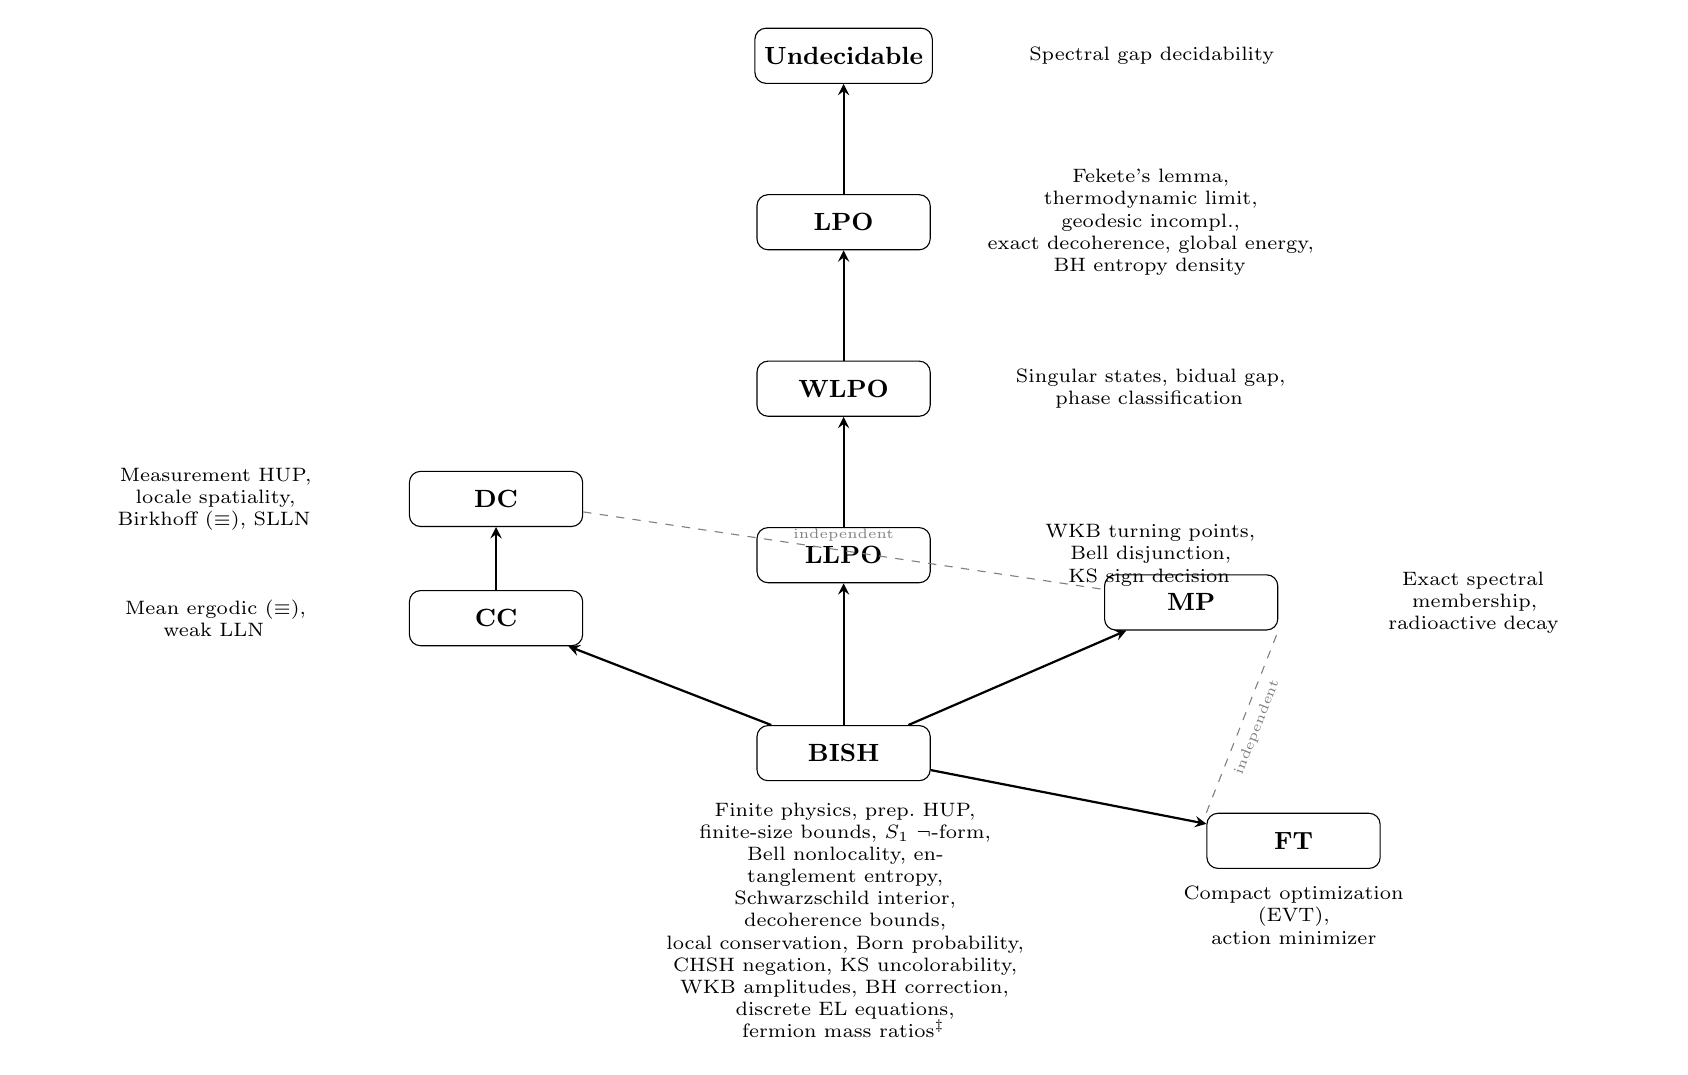
\begin{tikzpicture}[
  node distance=1.4cm and 2.8cm,
  principle/.style={draw, rounded corners, minimum width=2.2cm, minimum height=0.7cm, font=\small\bfseries},
  physlabel/.style={font=\scriptsize, text width=4.5cm, align=center},
  >=stealth
]
% Main spine (now includes LLPO)
\node[principle] (bish) {BISH};
\node[principle, above=1.8cm of bish] (llpo) {LLPO};
\node[principle, above=of llpo] (wlpo) {WLPO};
\node[principle, above=of wlpo] (lpo) {LPO};
\node[principle, above=of lpo] (undec) {Undecidable};

% Choice hierarchy (refined: CC < DC)
\node[principle, above left=1.0cm and 2.2cm of bish] (cc) {CC};
\node[principle, above=0.8cm of cc] (dc) {DC};
% Orthogonal branch
\node[principle, above right=1.2cm and 2.2cm of bish] (mp) {MP};

% Fan Theorem: independent branch
\node[principle, below right=0.4cm and 3.5cm of bish] (ft) {FT};

% Edges (Hasse diagram: only covering relations)
\draw[thick, ->] (bish) -- (cc);
\draw[thick, ->] (cc) -- (dc);
\draw[thick, ->] (bish) -- (mp);
\draw[thick, ->] (bish) -- (llpo);
\draw[thick, ->] (llpo) -- (wlpo);
\draw[thick, ->] (wlpo) -- (lpo);
\draw[thick, ->] (lpo) -- (undec);
\draw[thick, ->] (bish) -- (ft);

% Physical labels
\node[physlabel, below=0.15cm of bish] {Finite physics, prep.\ HUP,\\finite-size bounds, $S_1$ $\neg$-form,\\Bell nonlocality, entanglement entropy,\\Schwarzschild interior, decoherence bounds,\\local conservation, Born probability,\\CHSH negation, KS uncolorability,\\WKB amplitudes, BH correction,\\discrete EL equations,\\fermion mass ratios$^\ddagger$};
\node[physlabel, left=0.1cm of cc] {Mean ergodic ($\equiv$),\\weak LLN};
\node[physlabel, left=0.1cm of dc] {Measurement HUP,\\locale spatiality,\\Birkhoff ($\equiv$), SLLN};
\node[physlabel, right=0.1cm of mp] {Exact spectral\\membership,\\radioactive decay};
\node[physlabel, right=0.4cm of llpo] {\scriptsize WKB turning points,\\Bell disjunction,\\KS sign decision};
\node[physlabel, right=0.4cm of wlpo] {\scriptsize Singular states, bidual gap,\\phase classification};
\node[physlabel, right=0.4cm of lpo] {\scriptsize Fekete's lemma,\\thermodynamic limit,\\geodesic incompl.,\\exact decoherence, global energy,\\BH entropy density};
\node[physlabel, right=0.4cm of undec] {\scriptsize Spectral gap decidability};
\node[physlabel, below=0.1cm of ft] {Compact optimization\\(EVT),\\action minimizer};

% Independence annotations
\draw[dashed, gray] (dc) -- node[above, font=\tiny, gray] {independent} (mp);
\draw[dashed, gray] (ft.north west) -- node[below, font=\tiny, gray, sloped] {independent} (mp.south east);

\end{tikzpicture}%
}
\caption{The logical geography of mathematical physics (v5.0). Arrows indicate strict implication over BISH. The omniscience spine (BISH $<$ LLPO $<$ WLPO $<$ LPO) forms the dominant vertical chain. DC$_\omega$ and MP occupy orthogonal positions. The Fan Theorem (FT) constitutes a third independent branch: it neither implies nor is implied by any principle on the omniscience spine, and is independent of both DC$_\omega$ and MP. Physical layers are annotated with their calibrated logical cost.}
\label{fig:geography}
\end{figure}

\noindent$^\dagger$AxCal methodology --- assembly proof verified in Lean, mathematical prerequisites axiomatized as bridge lemmas. See \S\ref{sec:machine}. Paper~6 v2 has been upgraded to CRM (Mathlib-based) and no longer carries this designation.

\noindent$^\ddagger$Paper~18 is a numerical (Python) computation, not a Lean~4 formalization.

\textbf{New entries in v1.1.} Paper~11 extends the calibration from ``states, limits, spectra'' to ``tensor products, entanglement, correlations.'' The BISH results confirm that quantum compositional structure --- the infrastructure of entanglement itself --- carries no non-constructive cost. Paper~13 extends from statistical mechanics to gravitation: the Schwarzschild interior's finite-time physics is BISH, while geodesic incompleteness costs exactly LPO via BMC.

\textbf{New entries in v2.0.} Papers~14, 15, and~16 extend the calibration to quantum decoherence, conservation laws, and the Born rule. Paper~14 calibrates exact decoherence at LPO (third BMC domain). Paper~15 calibrates global energy at LPO (fourth BMC domain, first structural law). Paper~16 calibrates frequentist convergence at DC$_\omega$. Together these double the domain-invariance evidence from two to four BMC~$\equiv$~LPO instances and populate the DC$_\omega$ axis.

\textbf{New entries in v3.0.} Papers~17--24 extend the calibration to quantum gravity, particle physics, semiclassical mechanics, quantum foundations, and radioactive decay, while populating the previously empty LLPO level and establishing the Fan Theorem as a third independent branch.

Paper~17 [Lee 2026m] calibrates Bekenstein-Hawking entropy: algebraic correction is BISH, entropy density convergence costs LPO (fifth BMC domain --- quantum gravity). Paper~18 [Lee 2026n] applies the Scaffolding Principle to fermion masses: mass ratios are BISH; removing LPO scaffolding produces no new constraints (methodologically essential negative result; numerical Python computation). Paper~19 [Lee 2026o] calibrates WKB tunneling with a three-tier structure: amplitudes (BISH), turning-point existence (LLPO via IVT), semiclassical limit (LPO). This is the first physical LLPO calibration. Paper~20 [Lee 2026p] establishes observable-dependent logical cost: the 1D Ising model costs BISH, WLPO, LPO, or FT depending on the observable queried. Paper~21 [Lee 2026q] calibrates Bell nonlocality: CHSH violation is BISH, disjunctive conclusion costs LLPO (second LLPO calibration). Paper~22 [Lee 2026r] calibrates radioactive decay at MP (first physical MP calibration with both directions) and diagnoses the tunneling traversal time controversy as an MP disagreement. Paper~23 [Lee 2026s] calibrates compact optimization at FT (independent of the omniscience chain; zero custom axioms). Paper~24 [Lee 2026t] calibrates KS contextuality at LLPO (third LLPO calibration), detecting the structural identity Bell~$\equiv$~KS.

Together, these eight papers: (1)~populate LLPO with three independent calibrations, resolving v2.0 Problem~3a; (2)~establish the Fan Theorem as a third independent branch; (3)~demonstrate observable-dependent cost; and (4)~detect structural identities invisible to informal analysis.

\textbf{New entries in v4.0.} Paper~28 [Lee 2026v] extends the calibration to classical mechanics by establishing a constructive stratification between the Newtonian and Lagrangian formulations. For the discrete harmonic oscillator, the Euler-Lagrange equation is solvable in BISH (an explicit algebraic solution requiring no Fan Theorem), while the assertion that the discrete action functional attains its minimum on the configuration space is equivalent to the Fan Theorem. This is the second FT calibration and the first demonstration that the equation-of-motion content of a physical theory and its variational/optimization framing can be constructively separated: the equations are BISH, the optimization costs FT. The result strengthens the FT branch of the hierarchy, which previously contained only the abstract EVT result of Paper~23.

\textbf{New entries in v5.0.} Paper~29 [Lee 2026w] establishes that Fekete's Subadditive Lemma is equivalent to LPO over BISH: encoding a binary sequence $\alpha$ into a mock free energy $F_n = -n \cdot x_n$ (where $x_n = 1$ iff $\exists k < n, \alpha(k) = 1$) produces a subadditive sequence whose Fekete limit decides $\alpha$. This resolves Problem~1 (ineliminability) and identifies the generic mechanism behind the five-domain BMC~$\equiv$~LPO pattern: each domain produces a subadditive quantity, and Fekete's lemma is the tool that extracts its limit. The three-tier hierarchy for thermodynamic-limit convergence --- exact solvability (BISH), cluster expansion (BISH), generic subadditivity (LPO) --- explains why some models bypass LPO and others cannot.

The principal progression along the omniscience spine is monotone in the degree of physical idealization. The logical geography of physics is a partial order with the omniscience hierarchy (BISH $<$ LLPO $<$ WLPO $<$ LPO $<$ LEM) as its dominant spine, choice/decidability principles (DC$_\omega$, MP) providing lateral dimensions, and the Fan Theorem constituting a third independent branch rooted in compactness rather than omniscience.

\section{Background: Constructive Reverse Mathematics}

\subsection{The constructive hierarchy}

Bishop-style constructive mathematics (BISH) is mathematics carried out with intuitionistic logic and dependent choice, but without the law of excluded middle (LEM), the full axiom of choice, or any continuity principles. It is a common core: every BISH theorem is valid in classical mathematics, in recursive mathematics, and in Brouwerian intuitionism. The constructive hierarchy consists of principles that extend BISH by calibrated amounts:

\textbf{LLPO} (Lesser Limited Principle of Omniscience): For any binary sequence $\alpha : \mathbb{N} \to \{0,1\}$ with at most one term equal to~1, either all odd-indexed terms are~0 or all even-indexed terms are~0. Equivalently, LLPO asserts that the real numbers have a decidable sign: for every real $x$, either $x \leq 0$ or $x \geq 0$. LLPO is strictly between BISH and WLPO. It captures the cost of \emph{disjunction without constructive witness} --- being able to assert ``$A$ or $B$'' without being able to say which.

\textbf{WLPO} (Weak Limited Principle of Omniscience): For any binary sequence $\alpha : \mathbb{N} \to \{0,1\}$, either $(\forall n)(\alpha(n) = 0)$ or $\neg(\forall n)(\alpha(n) = 0)$. This is the weakest standard omniscience principle above LLPO. It asserts that ``all zeros'' is decidable --- not by producing a counterexample, but by deciding whether one exists.

\textbf{LPO} (Limited Principle of Omniscience): For any binary sequence $\alpha : \mathbb{N} \to \{0,1\}$, either $(\forall n)(\alpha(n) = 0)$ or $(\exists n)(\alpha(n) = 1)$. This is strictly stronger than WLPO. It asserts that a binary sequence either is identically zero or has a term equal to one --- a genuine dichotomy, not merely the negation of universality.

\textbf{MP} (Markov's Principle): If a binary sequence is not all zeros, then it has a term equal to~1. MP is independent of the omniscience spine: it neither implies nor is implied by WLPO.

\textbf{FT} (Fan Theorem): Every bar of a finitely branching tree with bounded height is uniform. Equivalently, every pointwise continuous function on a compact metric space is uniformly continuous. FT is independent of the omniscience chain and independent of MP. It captures the logical content of compactness arguments.

\textbf{LEM} (Law of Excluded Middle): For any proposition $P$, either $P$ or $\neg P$. Full classical logic.

The strict implications along the omniscience spine are: BISH $<$ LLPO $<$ WLPO $<$ LPO $<$ LEM. Each inclusion is proper. The Fan Theorem, MP, and DC$_\omega$ occupy positions independent of this spine.

These principles have a precise proof-theoretic location. Both WLPO and LPO require $\Sigma^0_1$ excluded middle (decidability of existential arithmetic statements), while full LEM requires excluded middle at all arithmetic levels. The omniscience hierarchy thus decomposes a specific fragment of the gap between intuitionistic and classical arithmetic.

\subsection{The methodology: constructive reverse mathematics}

Classical reverse mathematics (Friedman, Simpson) asks: which set-existence axioms are needed to prove the theorems of ordinary mathematics? The base theory is RCA$_0$ (recursive comprehension), and the programme classifies theorems by their equivalence to one of five standard systems.

Constructive reverse mathematics (CRM) asks the analogous question over BISH: which omniscience principles are needed? A CRM result takes the form ``Theorem~$T$ is equivalent to principle~$P$ over BISH,'' meaning (i) BISH + $P$ proves $T$, and (ii) BISH + $T$ proves $P$. The equivalence is proven in a classical metatheory --- this is essential and not a defect, just as Simpson's results are proven in ZFC.

The programme was initiated by Ishihara [1992, 2006] and developed by Bridges and V\^{\i}\c{t}\u{a} [2006], among others. Key results include the equivalence of LPO with bounded monotone convergence, of WLPO with the existence of infima of bounded sequences, of LLPO with the intermediate value theorem (Ishihara 2006), and of the Fan Theorem with the extreme value theorem (Berger 2005, Bridges and V\^{\i}\c{t}\u{a} 2006).

\subsection{Machine verification}\label{sec:machine}

A distinctive feature of this programme is its reliance on formal verification in Lean~4. The companion papers provide complete Lean formalizations totalling approximately 21,249 lines of code across twenty-two papers. The \texttt{\#print axioms} command provides a machine-checkable certificate that a given proof uses no classical axioms beyond those explicitly declared --- a level of assurance unavailable to pen-and-paper proofs about constructive validity.

\textbf{Methodological distinction.} The companion papers employ three distinct formalization methodologies. Papers~2, 5, 6, 7, 8, 9, 11, 13, 14, 15, 16, 17, 19, 20, 21, 22, 23, 24, 28, and~29 use \emph{CRM over Mathlib}. Paper~4 uses the \emph{AxCal framework} in mathlib-free Lean~4. Paper~18 uses numerical computation in Python. The calibration claims from all methodologies populate the table; the distinction in verification depth should be understood when interpreting the entries.

\section{Methodology: Formalization in a Classical Metatheory}\label{sec:methodology}

\subsection{The standard CRM methodology}

Constructive reverse mathematics has always operated within a classical metatheory. Bridges and Richman prove their equivalences using informal mathematics that implicitly includes excluded middle at the meta-level. Lean~4 with Mathlib is the classical metatheory. The constructive content is extracted by inspecting what the proofs actually use, as reported by \texttt{\#print axioms}.

\subsection{Three certification levels}

The formalizations in this series achieve different levels of certification:

\begin{enumerate}
\item \textbf{Mechanically certified.} The Lean build target compiles without \texttt{Classical.choice} in \texttt{\#print axioms}. Examples: Paper~2's P2\_Minimal and Paper~7's P7\_Minimal.

\item \textbf{Structurally verified.} \texttt{Classical.choice} is inherited from Mathlib infrastructure, but the proof uses only constructively valid reasoning. Examples: Papers~7, 8A, 9A, 11, 13 (BISH), 17 (BISH), 19 (BISH), 21 (BISH), 24 (BISH), 28 (BISH half).

\item \textbf{Intentional classical content.} The proof uses classical principles by design --- the classical content is the \emph{theorem}. Examples: Paper~8B (LPO), Paper~19 (LLPO), Paper~21 (LLPO), Paper~24 (LLPO), Paper~20 (WLPO), Paper~22 (MP), Paper~23 (FT), Paper~28 (FT half).
\end{enumerate}

\subsection{The Mathlib question}

Mathlib imports \texttt{Classical.em} and \texttt{Classical.choice} at the library level. These enter the axiom profile through typeclass resolution. The result: \texttt{\#print axioms} cannot distinguish between ``this theorem requires classical logic'' and ``this theorem's proof happens to be written in a library that assumes classical logic.'' This is the expected behavior of a classical metatheory.

A concrete illustration arises in papers that work over Mathlib's real numbers $\mathbb{R}$ (e.g., Papers~23, 28). Mathlib constructs $\mathbb{R}$ via classical Cauchy completion, so \texttt{Classical.choice} pervades the ambient type. Consequently, \texttt{\#print axioms} reports \texttt{[propext, Classical.choice, Quot.sound]} uniformly for \emph{all} theorems mentioning $\mathbb{R}$ --- including theorems whose proofs are purely algebraic (explicit witness construction, \texttt{field\_simp}, \texttt{linarith}). The constructive stratification in such papers is therefore established by the \emph{mathematical content} of the proofs, not by the axiom checker output: the BISH half uses only explicit algebraic manipulation and carries \texttt{FanTheorem} as no hypothesis, while the FT half proceeds by reduction to \texttt{FanTheorem} carried as a hypothesis. This is the same methodological situation as in standard CRM, where the metatheory is classical and the constructive content is established by inspecting what the proof actually uses.

\subsection{The role of minimal artifacts}

Where the constructive claim is non-trivial, the series provides dependency-free ``minimal'' artifacts. No minimal artifact is needed for BISH content involving finite-dimensional matrix algebra, explicit trigonometric evaluation, finite-sum manipulation, or exhaustive finite search (Paper~24's \texttt{native\_decide} over $2^{18}$ colorings).

\subsection{Limitations}

A fully constructive Lean library for CRM does not currently exist. Building one is a major infrastructure project beyond this series' scope. The methodology described above mirrors the standard practice in CRM where the metatheory is classical and the constructive content is established by mathematical argument.

\section{The Verified Results}

We summarize the companion papers that anchor the calibration table.

\subsection{The Bidual Gap equivalence (Paper~2)}

\textbf{Theorem} [Lee 2026a]. Over BISH, the following are equivalent: (i)~WLPO; (ii)~there exists a Banach space $X$ and a bidual-gap witness for $X$. The proof proceeds via the Ishihara kernel technique. Non-reflexivity itself has the exact logical strength of WLPO.

\subsection{The Physical Bidual Gap (Paper~7)}

\textbf{Theorem} [Lee 2026b]. $S_1(H)$ is not reflexive (BISH). Any bidual-gap witness for $S_1(H)$ implies WLPO. This anchors the abstract result of Paper~2 in the canonical state space of quantum mechanics.

\subsection{Dispensability of the thermodynamic limit (Paper~8, Part~A)}

\textbf{Theorem} [Lee 2026c, Part~A]. For the 1D Ising model, $|f_N(\beta) - f_\infty(\beta)| \leq N^{-1} \cdot \tanh(\beta J)^N$, provable in BISH. The empirical content of the thermodynamic limit is available without the idealization.

\subsection{The LPO cost of the thermodynamic limit (Paper~8, Part~B)}

\textbf{Theorem} [Lee 2026c, Part~B]. Over BISH: LPO $\Leftrightarrow$ BMC. Paper~8 instantiates this: the free energy densities form a bounded monotone sequence. Paper~9 re-derives both results combinatorially, confirming formulation-invariance.

\subsection{Quantum spectra calibration (Paper~4)}

Paper~4 calibrates five spectral scenarios spanning BISH (S0, S4), DC$_\omega$ (S2), MP (S1), and WLPO (S3). The spectral calibration reveals that MP is orthogonal to the omniscience hierarchy.

\subsection{Heisenberg uncertainty (Paper~6)}

Preparation uncertainty (HUP-RS) is BISH. Measurement uncertainty (HUP-M) costs DC$_\omega$.

\subsection{Quantum entanglement structure (Paper~11)}

Tsirelson bound, Bell state entropy, and partial trace are BISH. Quantum compositional structure carries no non-constructive cost.

\subsection{Schwarzschild interior (Paper~13)}

Finite-time physics (cycloid, Kretschner scalar) is BISH. Geodesic incompleteness costs LPO. The event horizon functions as a logical boundary.

\subsection{Quantum decoherence (Paper~14)}

Finite-step decoherence bounds are BISH. Exact decoherence costs LPO via ABC~$\equiv$~BMC. Third BMC domain.

\subsection{Noether's theorem (Paper~15)}

Local conservation is BISH. Global energy costs LPO via NPSC~$\equiv$~BMC. Fourth BMC domain. The sign of the conserved density is logically significant.

\subsection{The Born rule (Paper~16)}

Born probabilities and the Chebyshev bound are BISH. The SLLN costs DC$_\omega$.

\subsection{Bekenstein-Hawking entropy (Paper~17)}

Algebraic correction is BISH. Entropy density convergence costs LPO via BMC. Fifth BMC domain (quantum gravity).

\subsection{Fermion mass hierarchy (Paper~18)}

Mass ratios are BISH (numerical). The Scaffolding Principle produces no new constraints --- a methodologically essential negative result.

\subsection{WKB tunneling (Paper~19)}

Three-tier structure: amplitudes (BISH), turning-point existence (LLPO), semiclassical limit (LPO). First physical LLPO calibration.

\subsection{Observable-dependent logical cost (Paper~20)}

The 1D Ising model costs BISH, WLPO, LPO, or FT depending on the observable. Phase classification (magnetization zero-test) $\equiv$ WLPO.

\subsection{Bell nonlocality (Paper~21)}

CHSH violation (negation form) is BISH. Disjunctive conclusion costs LLPO. Second LLPO calibration.

\subsection{Markov's Principle and radioactive decay (Paper~22)}

``Non-zero decay rate implies eventual detection'' $\equiv$ MP. Tunneling traversal time controversy diagnosed as MP disagreement.

\subsection{Fan Theorem and compact optimization (Paper~23)}

EVT on $[a,b]$ $\equiv$ FT. Independent of the omniscience chain. Third independent branch. Zero custom axioms.

\subsection{Kochen-Specker contextuality (Paper~24)}

KS uncolorability (finite search) is BISH. KS sign decision $\equiv$ LLPO. Structural identity: Bell~$\equiv$~KS at LLPO.

\subsection{Newton vs.\ Lagrange: constructive stratification (Paper~28)}

Discrete Euler-Lagrange equations (BISH). Action minimizer existence $\equiv$ FT. Classical mechanics' Newtonian and Lagrangian formulations are constructively separated: the equation-of-motion content is BISH, the variational optimization framing costs FT. Second FT calibration.

\subsection{The choice axis: ergodic theorems and laws of large numbers (Paper~25)}

Mean Ergodic Theorem (von Neumann) $\equiv$ CC. Birkhoff's Ergodic Theorem $\equiv$ DC$_\omega$. Weak LLN $\leq$ CC. Strong LLN $\leq$ DC$_\omega$. The choice hierarchy AC$_0 < $ CC $ < $ DC$_\omega$ separates ensemble convergence (L$^2$) from pointwise a.e.\ convergence. A Type-level reverse direction is non-trivially formalized via a Prop/Type lifting technique (395 lines, hypothesis genuinely used). DC Ceiling Thesis: no calibrated physical theorem requires more than DC$_\omega$.

\section{The Programme's Development}

The preceding section catalogues the verified results as formal theorem statements. But the calibration table did not emerge from a single coordinated campaign; it grew through four distinct phases of investigation, each prompted by the discoveries and limitations of the phase before it. The Executive Summary (\S1) introduced each paper individually; here we trace how they relate to each other, how the programme's understanding evolved, and how the cumulative evidence reshaped the working hypothesis. The following account is necessarily retrospective --- the phases were not planned in advance --- but the trajectory they reveal is essential for understanding what the calibration table means and why it looks the way it does.

\subsection{The Pre-LPO Era: Axiom Calibration and First Probes (Papers~2, 4, 6, 7)}

Before the BMC~$\equiv$~LPO equivalence was discovered, the programme lacked its signature technique. The earliest papers explored whether constructive questions about physics were interesting at all, using a rudimentary approach we might call \emph{axiom calibration}: classifying what logical axioms a theorem uses, without establishing the tight equivalences that characterise constructive reverse mathematics proper. The question at this stage was not ``what is the exact logical cost?'' but the more basic ``does this question even have a non-trivial answer?''

\medskip

\textbf{Paper~2: The bidual gap (WLPO).} The programme's point of origin was a deceptively simple observation about bra-ket notation. When physicists write $\langle \phi | \psi \rangle$, they implicitly identify a Hilbert space with its double dual --- every continuous linear functional on functionals is assumed to come from a vector. What is the logical cost of this identification? The answer, obtained via the Ishihara kernel technique, is WLPO: the ability to decide ``all entries of an infinite binary sequence are zero'' versus ``not all are zero.'' The surprise was not that the cost was non-trivial --- this was expected --- but that it was \emph{specifically} WLPO rather than the stronger LPO. The identification is logically expensive, but not maximally so. This was the first indication that specific omniscience principles could be attached to specific pieces of physics, and that the attachment might be informative.

\textbf{Paper~4: Quantum spectra (BISH through WLPO, with MP orthogonal).} The spectral calibration was the most technically ambitious early paper. Five spectral scenarios for self-adjoint operators --- from approximate eigenvalues to exact spectral membership --- were classified at five different logical costs: BISH, DC$_\omega$, MP, and WLPO. The key insight was that MP (Markov's Principle: if a computation does not fail to halt, then it halts) turned out to be orthogonal to the omniscience hierarchy. This was the first evidence that the logical geography of physics is a partial order, not a linear chain. Methodologically, Paper~4 used the AxCal (Axiom Calibration) framework rather than CRM over Mathlib --- a lighter-weight approach that sacrificed some mathematical depth for logical transparency. The spectral calibration served as a roadmap: it showed that the hierarchy contained multiple levels and multiple axes, all waiting to be populated by physics.

\textbf{Paper~6: Heisenberg uncertainty (BISH).} The Heisenberg uncertainty principle is perhaps the most philosophically loaded result in quantum mechanics --- often invoked as evidence that quantum mechanics is fundamentally mysterious or non-classical. The discovery that preparation uncertainty (the Robertson-Schr\"odinger inequality) is pure BISH --- nothing but Cauchy-Schwarz geometry in finite-dimensional inner product spaces --- was both a relief and a validation. One of quantum mechanics' most philosophically loaded results requires no non-constructive logic whatsoever. The subtlety emerged in the distinction between preparation and measurement: measurement uncertainty costs DC$_\omega$, introducing a clean separation between quantum algebraic structure (BISH) and statistical inference about measurement outcomes (DC$_\omega$). Paper~6 in its second version (v2) upgraded from AxCal to CRM over Mathlib, establishing the technical standard that subsequent papers would follow.

\textbf{Paper~7: Trace-class operators (WLPO).} Paper~7 anchored Paper~2's abstract bidual result in the physically relevant setting of trace-class operators --- the density matrices that describe quantum states. The separation was sharp: ``singular states cannot be ruled out'' is BISH (a negative result), while ``a singular state can be explicitly exhibited'' requires WLPO (a positive construction). This crystallised the programme's central theme: the gap between negative and positive constructive results tracks the gap between what can be operationally excluded and what can be concretely produced. Physics routinely treats these as interchangeable; constructive analysis reveals they are not.

\medskip

\textbf{Phase assessment.} Phase~1 achieved proof of concept: specific omniscience principles attach to specific physics, and the attachment is non-trivial. But the approach was unsystematic. Most results were one-directional (``this theorem requires at least WLPO'') rather than equivalences (``this theorem is equivalent to WLPO over BISH''). The programme needed a canonical example where both directions of an equivalence could be proved cleanly --- a Rosetta Stone that would make the technique reproducible. That example arrived with Paper~8.

\subsection{The BISH-LPO Systematic Era: BMC Equivalence and Domain Expansion (Papers~8, 9, 11, 13, 14, 15)}

Paper~8 transformed the programme from an exploratory venture into a systematic calibration project. The discovery was that \emph{Bounded Monotone Convergence} (BMC) --- every bounded monotone sequence of real numbers converges --- is equivalent to LPO over BISH. Applied to the 1D Ising model, this gave the programme its paradigmatic result: the finite Ising model is BISH, the thermodynamic limit costs exactly LPO, and the equivalence is tight in both directions. For the first time, the programme possessed a clean, reproducible technique: encode a binary sequence into physical parameters, show that convergence of the physical quantity is equivalent to deciding the sequence, and thereby establish an exact calibration.

\medskip

\textbf{Paper~8: The 1D Ising model (BISH / LPO).} The physical question was elementary: what is the logical cost of taking the thermodynamic limit in the simplest statistical-mechanical model? The approach was to encode a binary sequence $\alpha$ into the coupling constants $J_n = J \cdot (1 - \alpha_n)$ of a one-dimensional Ising chain, making the free energy sequence's convergence equivalent to deciding whether $\alpha$ is eventually zero. Part~A showed that empirical predictions --- finite-size bounds with exponential error $|f_N - f_\infty| \leq N^{-1} \tanh(\beta J)^N$ --- are available in BISH, with no omniscience needed. Part~B showed that the completed limit costs exactly LPO via BMC. The surprise was not the LPO cost itself (completed limits being expensive is unsurprising) but the combination of \emph{dispensability} and \emph{exactness}: the non-constructive superstructure is genuinely dispensable for predictions (Part~A), yet the completed limit costs \emph{exactly} LPO, no more and no less (Part~B). The dispensability result was arguably more important than the cost result --- it showed that physics can be done constructively without losing empirical content. Paper~29 subsequently showed that this LPO cost is not specific to the 1D Ising encoding: Fekete's Subadditive Lemma itself is equivalent to LPO, establishing the cost as ineliminable for \emph{any} system whose thermodynamic limit proceeds through subadditivity.

\textbf{Paper~9: Formulation-invariance (BISH / LPO).} Paper~9 was the programme's first robustness test. The same physical quantity (the 1D Ising free energy density) was re-derived using purely combinatorial methods --- bond variables and the binomial parity sieve --- instead of the transfer-matrix eigenvalue decomposition of Paper~8. The axiom profiles were identical. This confirmed that the LPO cost is a property of the physics, not the mathematical machinery chosen to describe it. Formulation-invariance was essential for the programme's philosophical credibility: if the logical cost changed with the formalism, it would be an artifact of the representation rather than a property of the physical content.

\textbf{Paper~11: Quantum entanglement (BISH).} Paper~11 extended the calibration to quantum information theory. The motivating question was whether quantum entanglement --- the phenomenon Einstein dismissed as ``spooky action at a distance'' --- carries non-constructive cost. The answer was no: the Tsirelson bound $2\sqrt{2}$, Bell state entanglement entropy, and partial trace are all BISH. The non-constructive content enters through infinite-dimensional tensor-product completions, not through quantum correlations. This was a reassuring confirmation that the BISH base is broad: the entire compositional structure of finite-dimensional quantum mechanics --- the part that quantum computing actually uses --- is constructively innocent.

\textbf{Paper~13: The Schwarzschild interior (BISH / LPO).} Paper~13 was the programme's first venture into general relativity. The Schwarzschild interior's finite-time physics --- the cycloid trajectory of an infalling observer, the Kretschner curvature scalar at any finite radius --- is BISH. Geodesic incompleteness --- the assertion that the infalling worldline terminates in finite proper time at the singularity --- costs LPO via BMC. The event horizon coincides with the logical boundary: the surface where constructive mathematics can no longer describe the geometry is the same surface where the geometry itself becomes singular. This was the second independent BMC~$\equiv$~LPO domain, and the first evidence of \emph{domain invariance}: completely different physics (statistical mechanics vs.\ general relativity) producing the identical logical pattern (finite content BISH, completed limit LPO). The pattern was beginning to look systematic.

\textbf{Paper~14: Quantum decoherence (BISH / LPO).} Paper~14 calibrated quantum decoherence --- the process by which a quantum system loses coherence through interaction with its environment. Finite-step decoherence bounds (how much coherence is lost after $N$ environmental interactions) are BISH. Exact decoherence (complete loss of quantum coherence in the infinite-environment limit) costs LPO via a variant of BMC: alternating bounded convergence (ABC), which is provably equivalent to BMC over BISH. Third BMC domain. The measurement problem, in part, is a logical artifact: the controversy about whether wave function collapse ``really happens'' is entangled with the question of whether the infinite-environment limit that produces exact decoherence exists constructively.

\textbf{Paper~15: Noether's theorem (BISH / LPO).} Paper~15 calibrated one of the deepest results in mathematical physics: Noether's theorem relating continuous symmetries to conservation laws. Local conservation (the divergence-free current density) is BISH. Global energy existence --- the assertion that the integral of energy density over all of space converges to a definite real number --- costs LPO via another BMC variant: non-negative partial sum convergence (NPSC), equivalent to BMC over BISH. Fourth BMC domain. A methodological insight emerged: the \emph{sign} of the conserved density is logically significant. Non-negative partial sums converge by BMC, but partial sums that oscillate in sign may require strictly stronger principles. Physics does not always produce non-negative densities, and the logical difference matters.

\medskip

\textbf{Phase assessment.} Phase~2 established the programme's core paradigm: finite physics is BISH, completed infinite limits cost LPO, and the cost is both formulation-invariant (Paper~9) and domain-invariant (Papers~8, 13, 14, 15). The same BMC~$\equiv$~LPO equivalence governed four independent physical domains: statistical mechanics, general relativity, quantum decoherence, and conservation laws. Paper~29 later revealed the deeper reason: all four domains produce subadditive quantities, and Fekete's Subadditive Lemma --- the generic tool for extracting limits from subadditivity --- is itself equivalent to LPO. The pattern was unmistakable. But the picture was incomplete. The LLPO level between BISH and WLPO was empty --- no physical proposition had been calibrated there. The Fan Theorem had no physical instantiation. Markov's Principle had only a one-directional calibration (Paper~4 showed that exact spectral membership \emph{requires} MP, but did not establish the converse). The hierarchy appeared as a ladder with missing rungs. The question confronting the programme was whether those rungs genuinely did not exist in physics, or whether they were simply waiting to be discovered.

\subsection{Pushing to the Frontier: The Limits of CRM (Papers~16, 17, 18)}

With the BISH-LPO paradigm firmly established, Phase~3 asked a more ambitious question: could CRM illuminate genuinely enigmatic physics problems? Not just calibrate well-understood models like the 1D Ising chain, but provide new insight into the measurement problem, quantum gravity, and particle physics --- domains where foundational questions remain open. This phase found the boundary of what CRM can do. It produced one significant positive result (Paper~17), one genuinely new logical-level identification (Paper~16), and one methodologically essential negative result (Paper~18).

\medskip

\textbf{Paper~16: The Born rule (BISH / DC$_\omega$).} Paper~16 addressed the probabilistic interpretation of quantum mechanics. The Born rule --- the recipe that converts quantum amplitudes $|\langle \phi | \psi \rangle|^2$ into probabilities --- is the bridge between the formalism and experimental prediction. What is its logical cost? The answer contained a genuine surprise: Born probabilities and the Chebyshev bound (the finite weak law of large numbers) are BISH, but the strong law of large numbers (the assertion that relative frequencies converge to theoretical probabilities) requires DC$_\omega$ (dependent countable choice). This was significant for two reasons. First, it populated the DC$_\omega$ axis with a physically substantive entry --- previously, DC$_\omega$ had appeared only in the AxCal-based spectral calibration (Paper~4) and the relatively technical measurement-uncertainty result (Paper~6). Second, it provided a partial diagnosis of the measurement problem: the controversy over what quantum measurement ``really means'' is entangled with the question of whether infinite measurement sequences can be constructively assembled. The finite Born rule is uncontroversial; the infinite-frequency interpretation of probability is where the logical cost resides. Paper~16 also diagnosed the measurement problem as, in part, a \emph{disagreement about DC$_\omega$}, not merely about physics.

\textbf{Paper~17: Bekenstein-Hawking entropy (BISH / LPO).} Paper~17 extended the programme to quantum gravity --- specifically, the Bekenstein-Hawking area-entropy relation $S = A/4$ as derived from loop quantum gravity spin-network state counting. The algebraic logarithmic correction coefficient ($-3/2$) is BISH --- pure algebra, no omniscience. The entropy density convergence in the LQG state-counting sum costs LPO via BMC. This was the fifth independent BMC domain, and by far the most physically exotic: the same mathematical pattern that governs the 1D Ising model's thermodynamic limit also governs the convergence of black hole entropy in a candidate theory of quantum gravity. With domain invariance now established across five unrelated domains --- statistical mechanics, general relativity, quantum decoherence, conservation laws, and quantum gravity --- coincidence became increasingly implausible. The BMC~$\equiv$~LPO equivalence appeared to capture something fundamental about the logical cost of completed infinite limits in physics, regardless of the specific physical theory.

\textbf{Paper~18: The fermion mass hierarchy (BISH).} Paper~18 was a deliberate probe of what the programme had begun calling the ``Scaffolding Principle'' --- the hypothesis that removing non-constructive mathematical scaffolding from a physical argument might reveal new physical constraints or predictions. The target was the fermion mass hierarchy: do the mass ratios of quarks and leptons (a set of dimensionless numbers spanning five orders of magnitude) satisfy constraints that become visible when LPO-dependent reasoning is removed? The answer was: no. The mass ratios are BISH --- they are finite-dimensional numerical quantities that can be computed by straightforward arithmetic. Removing the non-constructive scaffolding produces nothing new; the idle machinery is genuinely idle. This was a negative result, but it was \emph{methodologically essential}: it defined the boundary of CRM's applicability. CRM is informative when the physics has a natural finite/infinite stratification (finite system versus infinite limit, finite measurements versus infinite frequency). It is uninformative when the physics is already finite and algebraic. Paper~18 also broke with the series' methodology: it was the only paper that used numerical computation (Python) rather than Lean~4 formalization, reflecting the fact that the result was computational rather than proof-theoretic.

\medskip

\textbf{Phase assessment.} Phase~3 delineated the programme's frontier. CRM works well when physics has a natural finite/infinite stratification: finite Ising model versus thermodynamic limit, finite measurements versus infinite frequency, finite horizon-penetration versus geodesic completion, finite environment versus infinite decoherence. It yields diminishing returns when the physics is already finite and algebraic (fermion mass ratios). The programme now had a clear picture of its domain of applicability --- and, crucially, an unresolved question: were the missing levels of the hierarchy (LLPO, FT, a tight MP equivalence) genuinely absent from the physics of the natural world, or simply undiscovered?

\subsection{Refinement, New Axes, and the Choice Hierarchy (Papers~19--25)}

Phase~4 was driven by the gaps in the hierarchy. The LLPO level --- strictly between BISH and WLPO on the omniscience spine --- had no physical instantiation. The Fan Theorem, capturing a mode of reasoning about compact spaces entirely independent of the omniscience chain, had no connection to physics. Markov's Principle lacked a two-directional physical equivalence. And the relationship between logical cost and physical system remained unexplored: was cost a property of the system, or of the question asked about it? Papers~19--25 answered all of these questions, and in doing so transformed the programme's understanding of the constructive hierarchy from a ladder with missing rungs into a tree with three independent branches and a refined choice axis. Paper~25 then opened a second axis entirely: the choice hierarchy CC $<$ DC, refining the DC$_\omega$ entries that had appeared since Phase~1 into a two-level structure where ensemble-level convergence (mean ergodic, weak LLN) requires only CC while individual-trajectory convergence (Birkhoff, strong LLN) requires the stronger DC.

\medskip

\textbf{Paper~19: WKB tunneling (BISH / LLPO / LPO).} Paper~19 calibrated semiclassical quantum tunneling through potential barriers using the WKB approximation. The result had a remarkably clean three-tier structure: specific transmission amplitudes for specific barriers are BISH (finite algebraic computation), the existence of a turning point for a general continuous potential costs LLPO (via the constructive intermediate value theorem), and the full semiclassical limit costs LPO (route-costed through BMC). This was the first physical LLPO calibration, resolving the ``LLPO gap'' that had been identified as Problem~3a in the previous version of this paper. The insight was structural: LLPO captures \emph{sign decisions} --- the ability to assert that a real number is non-negative or non-positive without specifying which. The turning point of a potential barrier is precisely such a sign decision: the point where $V(x) - E$ changes sign, asserted to exist without specifying on which side the transition occurs.

\textbf{Paper~20: Observable-dependent logical cost (BISH / WLPO / LPO / FT).} Paper~20 returned to the 1D Ising model --- already the most thoroughly calibrated system in the programme --- and made a discovery that changed the interpretation of the entire calibration table. The same physical system requires different logical principles depending on which observable is queried:

\begin{center}
\begin{tabular}{@{}ll@{}}
Finite-volume bounds & BISH (Paper~8A) \\
Phase classification (magnetization zero-test) & $\equiv$ WLPO (Paper~20) \\
Thermodynamic limit existence & $\equiv$ LPO (Paper~8B) \\
Parameter-space optimization & $\equiv$ FT (Paper~23)
\end{tabular}
\end{center}

\noindent This was a conceptual shift of the first order. Logical cost is not a property of the physical system; it is a property of the \emph{question asked} about the system. The calibration table does not classify systems --- it classifies questions. A single system can inhabit BISH, WLPO, LPO, and FT simultaneously, depending on what one asks of it. This sharpened the programme's philosophical claim: the constructive hierarchy tracks the physicist's layers of \emph{inquiry}, not merely the physicist's layers of idealisation.

\textbf{Paper~21: Bell nonlocality (BISH / LLPO).} Paper~21 calibrated Bell nonlocality --- the foundational result at the heart of quantum mechanics' departure from classical physics. The CHSH inequality violation --- the statement that no local hidden variable theory can reproduce quantum correlations --- is BISH in its negation form: the \emph{refutation} of local realism is constructive, requiring only finite algebra. But the \emph{disjunctive conclusion} --- ``either locality fails or realism fails'' --- costs exactly LLPO. The logical anatomy of Bell's theorem was laid bare: the surprise is not the violation itself (which is constructive) but the disjunction (which requires the ability to assert one of two alternatives without specifying which). This was the second physical LLPO calibration, and the pattern unified with Paper~19: both LLPO costs arise from \emph{disjunction without constructive witness}. LLPO was emerging as the natural logical cost of ``either-or'' conclusions in physics --- conclusions where one of two alternatives must hold, but no finite computation can determine which.

\textbf{Paper~22: Radioactive decay and Markov's Principle (MP).} Paper~22 calibrated a deceptively simple physical assertion: ``if a radioactive nucleus has a non-zero decay rate, it will eventually be detected as having decayed.'' This is equivalent to Markov's Principle --- the assertion that if a computation does not fail to halt, then it does halt --- with both directions proved. This was the first physical MP equivalence in the programme; Paper~4's spectral result had been one-directional. But the most striking result was \emph{diagnostic}: the tunneling traversal time controversy --- a genuine and unresolved disagreement among physicists about whether quantum tunneling takes a definite finite time --- was identified as a disagreement about MP. The different positions in the debate correspond to different commitments about whether the double negation ``it is not the case that the particle never arrives'' constructively implies ``the particle eventually arrives.'' CRM was functioning not merely as a calibration instrument for known physics, but as a \emph{diagnostic tool} for resolving (or at least clarifying) genuine physical controversies.

\textbf{Paper~23: The Fan Theorem and compact optimisation (FT).} Paper~23 calibrated compact optimisation --- the extreme value theorem asserting that a continuous function on a closed bounded interval attains its maximum --- at the Fan Theorem. FT is independent of the entire omniscience chain (BISH through LPO), independent of DC$_\omega$, and independent of MP. It captures a fundamentally different mode of reasoning: \emph{compactness} rather than convergence or disjunction. With this result, the hierarchy was definitively established as a tree with three mutually independent branches: the omniscience spine (BISH $<$ LLPO $<$ WLPO $<$ LPO), the choice and decidability axes (DC$_\omega$, MP), and the compactness branch (FT). Different classes of physical reasoning --- convergence arguments, disjunction arguments, compactness arguments --- draw on different, mutually independent logical wells. The formalization used zero custom axioms: every step was derived entirely from Mathlib's existing library, making it the cleanest CRM result in the entire series.

\textbf{Paper~24: Kochen-Specker contextuality (BISH / LLPO).} Paper~24 calibrated the Kochen-Specker theorem --- a fundamental no-go result in quantum foundations asserting that quantum observables cannot all be simultaneously assigned definite values in a context-independent manner --- and in doing so revealed a structural identity invisible to informal analysis. The KS uncolorability result (the finite combinatorial fact that no consistent value assignment exists for a specific set of projection operators) is BISH. The contextuality conclusion (the disjunctive ``either non-contextual hidden variables fail or value-definiteness fails'') costs exactly LLPO. This was the third LLPO calibration, and it mirrored Paper~21's Bell result exactly in logical structure. But the physical content is entirely different: Bell nonlocality involves spatially separated systems and the failure of locality; KS contextuality involves a single system and the failure of non-contextual value assignments. Yet both cost LLPO for the same structural reason --- \emph{disjunction without constructive witness}. CRM had detected a hidden structural identity: two physically unrelated no-go theorems, discovered independently and usually discussed in different chapters of quantum foundations textbooks, are the same logical phenomenon in different physical clothing.

\textbf{Paper~25: The choice axis (CC / DC).} Paper~25 opened a second axis in the calibration, largely orthogonal to the omniscience spine. The mean ergodic theorem (von Neumann, 1932) --- the assertion that time averages of a unitary operator converge in $L^2$ norm to the orthogonal projection onto the fixed subspace --- is equivalent to Countable Choice (CC) over BISH. Birkhoff's pointwise ergodic theorem --- the stronger assertion that time averages converge pointwise almost everywhere --- is equivalent to the stronger Dependent Choice (DC). The separation is physically clean: ensemble-level behavior (L$^2$ averages) requires CC; individual-trajectory behavior (pointwise convergence) requires DC. The weak and strong laws of large numbers calibrate correspondingly: weak LLN to CC, strong LLN to DC. This refines the existing DC$_\omega$ entries into a two-level choice hierarchy and establishes a DC Ceiling Thesis: no calibrated physical theorem in the programme requires more than DC.

\textbf{Paper~28: Newton vs.\ Lagrange (BISH / FT).} Paper~28 extended the programme to classical mechanics by establishing a constructive stratification between the Newtonian and Lagrangian formulations. For the discrete harmonic oscillator with two time steps, the Euler-Lagrange equation reduces to a scalar linear equation with an explicit algebraic solution --- pure BISH, no Fan Theorem. But the assertion that the discrete action functional attains its minimum on the configuration space is equivalent to the Fan Theorem via the extreme value theorem on $[0,1]$. The significance is twofold. First, this is the second independent FT calibration, strengthening the FT branch that Paper~23 had established with only one entry. Second, and more novel, it demonstrates that two formulations of the \emph{same} physical law --- the Newtonian equation-of-motion approach and the Lagrangian variational approach --- can be constructively separated: the equations are BISH, the optimization is FT. The variational interpretation of classical mechanics is logically dispensable; the equations of motion are the physical content.

\medskip

\textbf{Phase assessment.} Phase~4 resolved every gap identified in earlier versions. LLPO was populated (Papers~19, 21, 24). FT was established as independent (Papers~23, 28). MP was tightened (Paper~22). Observable-dependent cost was discovered (Paper~20). CRM was shown to detect structural identities (Bell~$\equiv$~KS at LLPO) invisible to informal analysis. And Paper~25 opened a second axis --- the choice hierarchy CC $<$ DC --- refining the DC$_\omega$ entries into a two-level structure and calibrating ergodic theory against the choice principles. Paper~28 provided the second FT calibration and revealed a new dimension of the programme: constructive separation between \emph{formulations} of the same law, not merely between finite and infinite layers. The hierarchy was revealed as a tree with three branches and a refined choice axis, where each branch captured a different \emph{mode of reasoning} about the physical world --- convergence, disjunction, compactness, and choice. The calibration table was no longer a list of isolated curiosities; it was beginning to reveal the logical architecture of mathematical physics.

\subsection{Beyond Calibration}

The four phases traced above were not planned in advance. Each was prompted by the results and limitations of the phase before it: the pre-LPO explorations revealed that constructive analysis of physics was interesting; the BMC~$\equiv$~LPO discovery made it systematic; the frontier papers defined its boundaries; and the refinement papers revealed its depth. But the cumulative trajectory discloses an aspiration that transcends calibration: to understand how logic actually functions in the physical world.

The early papers (Phase~1) asked what logical axioms physics uses. The middle papers (Phases~2 and~3) established that the costs are intrinsic (formulation-invariant), reproducible (domain-invariant across five independent domains), and bounded (the frontier is identifiable). The late papers (Phase~4) revealed that the costs classify \emph{questions} rather than systems, and that CRM can detect structural identities invisible to informal analysis. At each stage, the programme moved from passive classification toward an active instrument for understanding the logical structure of physical theories.

Four phenomena, taken together, point beyond calibration toward something deeper. First, \emph{domain invariance}: the same BMC~$\equiv$~LPO equivalence governs completed limits in five unrelated physical domains --- unified by Paper~29's identification of Fekete's Subadditive Lemma ($\equiv$ LPO) as the common mechanism --- suggesting the cost is a property of the idealisation of infinite completion itself, not of any particular physical theory. Second, \emph{structural identity}: Bell nonlocality and KS contextuality share the LLPO cost for structural reasons (both are disjunctions without constructive witness), not by coincidence --- CRM reveals a kinship that decades of informal analysis did not detect. Third, \emph{diagnostic power}: CRM resolves genuine physical controversies (the tunneling traversal time debate is an MP disagreement; the measurement problem involves DC$_\omega$). Fourth, \emph{observable-dependence}: the logical structure tracks the physics finely enough to distinguish different observables within a single system, classifying the physicist's questions with a precision that system-level classifications cannot achieve. Fifth, \emph{choice-axis refinement}: Paper~25's separation of CC from DC shows that the choice hierarchy is not monolithic --- ensemble convergence and individual convergence draw on different levels of the same axis, and the separation tracks a genuine physical distinction between L$^2$ and pointwise-a.e.\ behavior. Sixth, \emph{formulation stratification}: Paper~28 demonstrates that two formulations of the same physical law --- Newtonian equations of motion and Lagrangian variational principles --- are constructively separated (BISH vs.\ FT), establishing that the logical cost attaches not only to the physics but to the \emph{framing} of the physics.

Whether these phenomena point to a deeper structural role for logic in physics --- whether the constructive hierarchy is not merely a mathematical taxonomy applied to physics but a reflection of the logical structure of physical reality itself --- is the question that the remaining sections, the correlation analysis, the working hypothesis, and the open problems, attempt to address.

\section{The Correlation and Its Significance}

\subsection{The pattern}

Assembling the results:

\textbf{BISH level.} Finite-volume quantum mechanics, preparation uncertainty, quantum compositional structure, Schwarzschild curvature and interior finite-time physics, finite-step decoherence, local conservation, Born probabilities, BH algebraic correction, WKB amplitudes, CHSH violation (negation form), KS uncolorability, and fermion mass ratios$^\ddagger$ are fully constructive. No omniscience or choice principle is needed.

\textbf{DC$_\omega$ level.} Measurement uncertainty, locale spatiality, and frequentist convergence (SLLN) require DC$_\omega$. These are the first costs incurred when moving from finite operational procedures to infinite data streams.

\textbf{LLPO level.} WKB turning-point decisions (Paper~19), Bell's disjunctive conclusion (Paper~21), and KS sign decisions (Paper~24) cost exactly LLPO. All three share the structure of \emph{disjunction without constructive witness}. LLPO is strictly between BISH and WLPO, and its three independent instantiations confirm that nature does not skip this level.

\textbf{MP level (orthogonal axis).} Exact spectral membership (Paper~4) and radioactive decay (Paper~22) require MP. The MP axis captures a distinct aspect of idealization --- the unbounded search needed to convert double-negation existence into constructive existence.

\textbf{WLPO level.} Singular states / bidual gap (Papers~2, 7), non-separable spectral separation (Paper~4), and phase classification (Paper~20) require WLPO.

\textbf{FT level (independent branch).} Compact optimization / EVT (Paper~23) and action minimizer existence in classical mechanics (Paper~28) require the Fan Theorem. FT is independent of the omniscience spine, MP, and DC$_\omega$. It captures compactness rather than convergence or disjunction. Paper~28 provides the second FT calibration and demonstrates that the variational formulation of classical mechanics is constructively stronger than the equation-of-motion formulation. This establishes the geography as a \emph{tree} with three independent branches.

\textbf{LPO level.} The thermodynamic limit (Papers~8, 9), geodesic incompleteness (Paper~13), exact decoherence (Paper~14), global energy (Paper~15), BH entropy density (Paper~17), and WKB semiclassical limit (Paper~19, route-costed) all cost LPO. Five independent domains produce subadditive quantities; Fekete's lemma ($\equiv$ LPO, Paper~29) is the generic extraction mechanism, with BMC as its proof-theoretic vehicle.

\textbf{Undecidable level.} The spectral gap problem is undecidable [Cubitt et al.\ 2015].

\begin{figure}[ht]
\centering
\resizebox{\textwidth}{!}{%
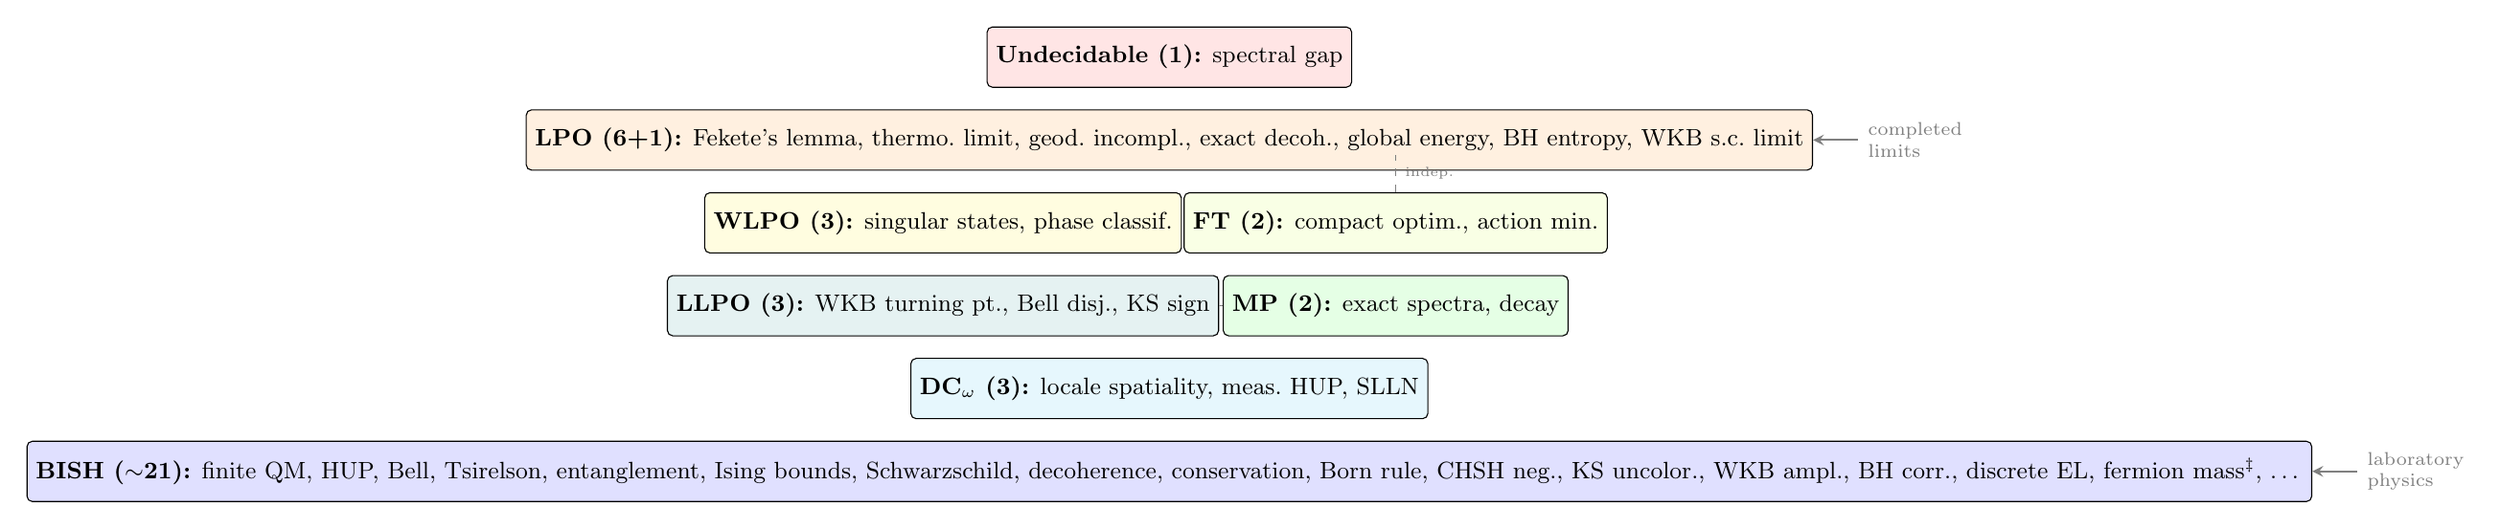
\begin{tikzpicture}[
  level/.style={draw, minimum height=0.8cm, rounded corners=2pt, font=\small,
    align=center},
  >=stealth
]
% Pyramid layers
\node[level, fill=blue!12, minimum width=13cm] (bish) at (0,0)
  {\textbf{BISH ($\sim$21):} finite QM, HUP, Bell, Tsirelson, entanglement,
   Ising bounds, Schwarzschild, decoherence, conservation, Born rule, CHSH neg., KS uncolor., WKB ampl., BH corr., discrete EL, fermion mass$^\ddagger$, \ldots};
\node[level, fill=cyan!10, minimum width=6cm] (dc) at (0,1.1)
  {\textbf{DC$_\omega$ (3):} locale spatiality, meas.\ HUP, SLLN};
\node[level, fill=teal!10, minimum width=5cm] (llpo) at (-3,2.2)
  {\textbf{LLPO (3):} WKB turning pt., Bell disj., KS sign};
\node[level, fill=green!10, minimum width=3.2cm] (mp) at (3,2.2)
  {\textbf{MP (2):} exact spectra, decay};
\node[level, fill=yellow!12, minimum width=4cm] (wlpo) at (-3,3.3)
  {\textbf{WLPO (3):} singular states, phase classif.};
\node[level, fill=lime!10, minimum width=3.5cm] (ft) at (3,3.3)
  {\textbf{FT (2):} compact optim., action min.};
\node[level, fill=orange!12, minimum width=8cm] (lpo) at (0,4.4)
  {\textbf{LPO (6+1):} Fekete's lemma, thermo.\ limit, geod.\ incompl., exact decoh., global energy, BH entropy, WKB s.c.\ limit};
\node[level, fill=red!10, minimum width=3cm] (undec) at (0,5.5)
  {\textbf{Undecidable (1):} spectral gap};

\draw[<-, thick, gray] (bish.east) -- +(0.6,0) node[right, font=\scriptsize, gray, align=left] {laboratory\\physics};
\draw[<-, thick, gray] (lpo.east) -- +(0.6,0) node[right, font=\scriptsize, gray, align=left] {completed\\limits};

\draw[dashed, gray] (llpo.east) -- node[above, font=\tiny, gray] {} (mp.west);
\draw[dashed, gray] (ft.north) -- node[right, font=\tiny, gray] {indep.} +(0,0.5);

\end{tikzpicture}%
}
\caption{Distribution of calibrated entries across logical levels (v5.0). The wide BISH base contains all finite-system, finite-time, and finite-sample physics. Three LLPO entries populate the level between BISH and WLPO. The Fan Theorem branch contains two independent calibrations. Paper~29 adds Fekete's Subadditive Lemma ($\equiv$ LPO) as the generic mechanism underlying the five-domain LPO pattern.}
\label{fig:pyramid}
\end{figure}

\subsection{Observable-dependent logical cost}

Paper~20 reveals that the same physical system can require different logical principles depending on which observable is queried. The 1D Ising model exhibits four distinct logical costs:

\begin{center}
\begin{tabular}{@{}ll@{}}
\toprule
Observable / Question & Logical Cost \\
\midrule
Finite-volume bounds & BISH (Paper~8A) \\
Phase classification (magnetization zero-test) & $\equiv$ WLPO (Paper~20) \\
Thermodynamic limit existence & $\equiv$ LPO (Paper~8B) \\
Parameter-space optimization & $\equiv$ FT (Paper~23) \\
\bottomrule
\end{tabular}
\end{center}

\noindent Logical cost is a property of the \emph{question asked}, not of the physical system.

\subsection{Structural identity detection}

Papers~21 and~24 reveal that CRM can detect structural identities invisible to informal analysis. Bell nonlocality and KS contextuality are physically distinct: the former involves spatially separated systems, the latter a single system. Yet both cost LLPO for the same reason --- disjunction without constructive witness. CRM identifies them as the same logical phenomenon in different physical clothing.

\subsection{Diagnostic power}

Paper~22 diagnoses the tunneling traversal time controversy as an MP disagreement. Paper~16 diagnoses the measurement problem (in part) as a DC$_\omega$ disagreement. CRM serves as a diagnostic instrument, revealing that apparent physical controversies are actually disagreements about logical commitments.

\subsection{Why this demands explanation}

The correlation is not between logical strength and mathematical generality --- it is between logical strength and \emph{physical idealization}. There is no a priori reason why the constructive hierarchy should track the layers of physical idealization.

\subsection{Comparison with van Wierst}

Van Wierst [2019] argued that constructive mathematics forces ``de-idealizations.'' Our contribution is to supply the precise logical price tags: the thermodynamic limit costs \emph{exactly} LPO, singular states cost \emph{exactly} WLPO, and the disjunctive consequences of no-go theorems cost \emph{exactly} LLPO.

\subsection{Comparison with Batterman}

Batterman [2005, 2011] argued that infinite idealizations are sometimes ``explanatorily essential.'' Our results sharpen the debate: predictions are BISH, explanations requiring completed limits cost LPO.

\subsection{Comparison with Pour-El and Richards}

Pour-El and Richards [1989] showed computable initial data can evolve non-computably. Our results address a different layer: the \emph{spaces} themselves have non-computable structure. Together, computability constraints on physics are severe at multiple levels.

\section{The Working Hypothesis}

\subsection{Statement}

\textbf{Working Hypothesis (Logical Geography).} In the constructive reverse mathematics of mathematical physics, all non-constructive costs arise from infinite-dimensional idealization layers --- not from the finite-dimensional or finite-time physical content. Empirical predictions are BISH-derivable. Moreover, different classes of physical reasoning require different, mutually independent logical resources: convergence arguments draw on LPO, disjunction arguments on LLPO, sign-test arguments on WLPO, compactness arguments on FT, ensemble-choice arguments on CC, individual-trajectory-choice arguments on DC, and unbounded-search arguments on MP.

The evidence now spans eleven domains: functional analysis, statistical mechanics, quantum information, general relativity, quantum measurement/decoherence, conservation laws, quantum gravity, quantum foundations, semiclassical/nuclear physics, ergodic theory, and classical mechanics (Paper~28: Newtonian EL equations = BISH, Lagrangian action minimization = FT).

Papers~8, 13, 14, 15, and~17 demonstrate the BMC~$\equiv$~LPO pattern in five independent physical domains. Paper~29 identifies the generic mechanism: Fekete's Subadditive Lemma is equivalent to LPO, explaining why all five domains --- each producing a subadditive quantity --- share the same logical cost.

This is not operationalism. We observe that the mathematical formulation of physics requires specific logical principles, and hypothesize that these principles track the boundary between the physically realizable and the mathematically ideal.

\subsection{Distinguishing features}

The hypothesis makes four claims: (1)~\emph{completeness} (every empirical prediction is BISH-derivable); (2)~\emph{monotonicity} (cost increases with idealization along the omniscience spine); (3)~\emph{formulation-invariance} (costs are properties of the physics); and (4)~\emph{observable-dependence} (cost depends on the question, not just the system).

\subsection{Relation to the Church-Turing thesis}

Our hypothesis is both more and less demanding than the Church-Turing thesis as a physical principle. BISH is stricter than Turing computability (requiring proofs of totality), but we require only that empirical content be expressible in BISH.

\subsection{Relation to Gisin's intuitionistic physics}

Gisin [2020, 2021] argued for ``intuitionistic physics.'' Our results supply the price tag. The positive news: quantum entanglement, finite-time GR, Born probabilities, local conservation, and CHSH violations are already intuitionistic. The reconstruction challenge lies at LLPO, WLPO, and LPO.

\section{The Formulation-Invariance Test}

Paper~9 re-derives both results of Paper~8 using purely combinatorial methods. The LPO cost is identical across formulations.

\subsection{Domain invariance: Papers 8, 13, 14, 15, and 17}

The same BMC~$\equiv$~LPO equivalence appears in five unrelated physical domains, unified by Paper~29's identification of Fekete's Subadditive Lemma as the generic underlying principle ($\equiv$ LPO):

\begin{itemize}
\item Paper~8: coupling constants $\to$ free energy $\to$ BMC.
\item Paper~13: geodesic data $\to$ proper time $\to$ BMC.
\item Paper~14: rotation angle $\to$ coherence $\to$ ABC ($\equiv$ BMC).
\item Paper~15: energy densities $\to$ partial sums $\to$ NPSC ($\equiv$ BMC).
\item Paper~17: puncture data $\to$ entropy density $\to$ BMC.
\end{itemize}

\begin{figure}[ht]
\centering
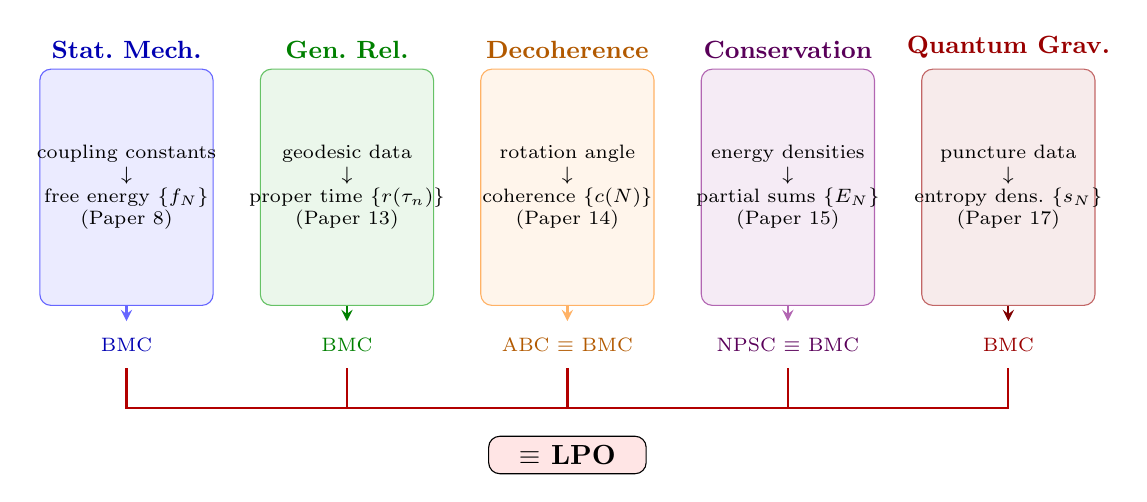
\begin{tikzpicture}[
  pillar/.style={draw, rounded corners, minimum width=2.2cm, minimum height=3cm,
    fill=#1!8, draw=#1!60},
  plabel/.style={font=\small\bfseries, #1},
  >=stealth
]
\node[pillar=blue] (sm) at (0,0) {};
\node[plabel=blue!70!black, above] at (sm.north) {Stat.\ Mech.};
\node[font=\scriptsize, align=center] at (sm.center) {coupling constants\\$\downarrow$\\free energy $\{f_N\}$\\(Paper~8)};

\node[pillar=green!60!black] (gr) at (2.8,0) {};
\node[plabel=green!50!black, above] at (gr.north) {Gen.\ Rel.};
\node[font=\scriptsize, align=center] at (gr.center) {geodesic data\\$\downarrow$\\proper time $\{r(\tau_n)\}$\\(Paper~13)};

\node[pillar=orange] (dc) at (5.6,0) {};
\node[plabel=orange!70!black, above] at (dc.north) {Decoherence};
\node[font=\scriptsize, align=center] at (dc.center) {rotation angle\\$\downarrow$\\coherence $\{c(N)\}$\\(Paper~14)};

\node[pillar=violet] (cl) at (8.4,0) {};
\node[plabel=violet!70!black, above] at (cl.north) {Conservation};
\node[font=\scriptsize, align=center] at (cl.center) {energy densities\\$\downarrow$\\partial sums $\{E_N\}$\\(Paper~15)};

\node[pillar=red!60!black] (qg) at (11.2,0) {};
\node[plabel=red!60!black, above] at (qg.north) {Quantum Grav.};
\node[font=\scriptsize, align=center] at (qg.center) {puncture data\\$\downarrow$\\entropy dens.\ $\{s_N\}$\\(Paper~17)};

\node[font=\scriptsize, blue!70!black] at (0,-2) {BMC};
\node[font=\scriptsize, green!50!black] at (2.8,-2) {BMC};
\node[font=\scriptsize, orange!70!black] at (5.6,-2) {ABC $\equiv$ BMC};
\node[font=\scriptsize, violet!70!black] at (8.4,-2) {NPSC $\equiv$ BMC};
\node[font=\scriptsize, red!60!black] at (11.2,-2) {BMC};

\draw[->, thick, blue!60] (sm.south) -- (0,-1.7);
\draw[->, thick, green!50!black] (gr.south) -- (2.8,-1.7);
\draw[->, thick, orange!60] (dc.south) -- (5.6,-1.7);
\draw[->, thick, violet!60] (cl.south) -- (8.4,-1.7);
\draw[->, thick, red!50!black] (qg.south) -- (11.2,-1.7);

\draw[thick, red!70!black] (0,-2.3) -- (0,-2.8) -- (11.2,-2.8) -- (11.2,-2.3);
\draw[thick, red!70!black] (2.8,-2.3) -- (2.8,-2.8);
\draw[thick, red!70!black] (5.6,-2.3) -- (5.6,-2.8);
\draw[thick, red!70!black] (8.4,-2.3) -- (8.4,-2.8);
\node[draw, rounded corners, fill=red!10, font=\bfseries, minimum width=2cm] at (5.6,-3.4) {$\equiv$ LPO};

\end{tikzpicture}
\caption{Domain invariance of BMC~$\equiv$~LPO (v5.0). Five independent physical domains each produce a subadditive quantity whose completed-limit existence costs exactly LPO. Paper~29 identifies Fekete's Subadditive Lemma ($\equiv$ LPO) as the generic mechanism: subadditivity is the common mathematical structure, with BMC as the proof-theoretic vehicle for extracting the limit.}
\label{fig:domain-invariance}
\end{figure}

\subsection{Formulation stratification: Paper~28}

Paper~28 reveals the complement of formulation-invariance: two formulations of the \emph{same} physical law can have \emph{different} constructive costs. The Newtonian formulation (solving the Euler-Lagrange equation) is BISH; the Lagrangian formulation (asserting the action attains its minimum) costs FT. Unlike Papers~8 and~9, where two mathematical routes to the same physical answer yield the same cost, Paper~28 shows that two \emph{conceptual framings} --- ``solve the equation'' versus ``minimize the functional'' --- yield different costs. The equation-of-motion content is the physical core; the variational interpretation is logically dispensable mathematical superstructure.

\subsection{The topos-theoretic alternative}

The precise relationship between the D\"oring-Isham internal logic and the BISH/LLPO/WLPO/LPO hierarchy has not been worked out. We flag this as a high-priority question.

\section{Open Problems}

Problems marked \textbf{[Resolved]} have been addressed by Papers~17--25.

\textbf{Problem~1.} \emph{Ineliminability.} \textbf{[Resolved by Paper~29.]} Fekete's Subadditive Lemma is equivalent to LPO over BISH (Paper~29). Since the thermodynamic limit proceeds via subadditivity of the log-partition function, the LPO cost is ineliminable for any system that lacks an explicit closed-form or cluster-expansion modulus. The three-tier hierarchy is: exact solvability (BISH), cluster expansion (BISH), generic subadditivity via Fekete (LPO).

\textbf{Problem~2.} \emph{Phase transitions without limits.} Can phase transitions be characterized constructively?

\textbf{Problem~3.} \emph{Intermediate and orthogonal principles.} \textbf{[Partially resolved.]} (a)~LLPO gap: \textbf{SOLVED} by Papers~19, 21, 24. (b)~DC$_\omega$ sharpness: \textbf{[Partially resolved]} by Paper~25, which separates CC from DC via ergodic theory; full sharpness of measurement-uncertainty calibration (whether CC suffices) remains open. (c)~MP formulation-invariance: \emph{Open.}

\textbf{Problem~4.} \emph{D\"oring-Isham calibration.} What is the constructive strength of the Bohrification topos?

\textbf{Problem~5.} \emph{Formulation-invariance for the WLPO level.} Does the C*-algebraic formulation yield the same cost?

\textbf{Problem~6.} \emph{Beyond statistical mechanics.} \textbf{[Partially resolved.]} Papers~17--25 extend to quantum gravity, particle physics, semiclassical mechanics, quantum foundations, radioactive decay, and ergodic theory. Renormalization group and UV limits remain open.

\textbf{Problem~7.} \emph{Infinite-dimensional entanglement entropy.} Does passage to infinite-dimensional entanglement introduce new costs?

\textbf{Problem~8.} \emph{Singularity calibration beyond Schwarzschild.} \textbf{[Partially addressed]} by Paper~17. Does the Penrose theorem calibrate above LPO?

\textbf{Problem~9.} \emph{SLLN calibration sharpness.} \textbf{[Resolved]} by Paper~25: DC is necessary for the SLLN (strong law calibrates to DC via Birkhoff's ergodic theorem). The weak law requires only CC.

\textbf{Problem~10.} (New.) \emph{Observable-dependent cost generality.} Does every multi-observable system exhibit observable-dependent cost?

\textbf{Problem~11.} (New.) \emph{LLPO completeness.} Are all physical LLPO calibrations sign decisions? Or can LLPO arise from a fundamentally different mechanism?

\textbf{Problem~12.} (New.) \emph{Fan Theorem physical population.} \textbf{[Partially resolved]} by Paper~28 (action minimizer existence $\equiv$ FT). What other physical assertions require FT? Does the variational formulation of every classical field theory cost FT?

\textbf{Problem~13.} (New.) \emph{Structural identity scope.} Do all quantum no-go theorems with disjunctive conclusions share the LLPO cost?

\textbf{Problem~14.} (New.) \emph{Scaffolding Principle testability.} In which domains does removing non-constructive scaffolding reveal new physics?

\textbf{Problem~15.} (New.) \emph{Choice-axis completeness.} Are there physical theorems that require exactly AC$_0$ (finite choice only)? Does the hierarchy AC$_0 < $ CC $ < $ DC have further physically calibratable intermediate levels?

\textbf{Problem~16.} (New.) \emph{Formulation stratification generality.} Paper~28 demonstrates that the Newtonian and Lagrangian formulations of classical mechanics are constructively separated (BISH vs.\ FT). Is this an isolated phenomenon, or does every variational formulation of a physical theory cost more than its equation-of-motion formulation? Does the Hamiltonian formulation introduce yet another logical level?

\section{Conclusion}

The constructive hierarchy of omniscience and choice principles turns out to map onto the layers of physical idealization in mathematical physics with surprising fidelity. Finite physics, preparation uncertainty, quantum entanglement structure, Schwarzschild finite-time physics, decoherence bounds, local conservation laws, Born probabilities, CHSH violations, KS uncolorability, WKB amplitudes, BH corrections, and discrete Euler-Lagrange equations are BISH. The mean ergodic theorem costs exactly Countable Choice (CC); Birkhoff's ergodic theorem costs Dependent Choice (DC). The weak law of large numbers sits at CC; the strong law at DC. Measurement uncertainty, spectral locale extraction, and frequentist convergence cost DC. WKB turning-point decisions, Bell disjunction, and KS sign decisions cost LLPO. Exact spectral membership and radioactive decay cost MP. The singular sector and phase classification cost WLPO. Compact optimization and action minimizer existence cost FT. The thermodynamic limit, geodesic incompleteness, exact decoherence, global energy, and BH entropy density cost LPO. The spectral gap is undecidable. The landscape is a partial order with three independent branches and a refined choice axis: the omniscience spine (BISH $<$ LLPO $<$ WLPO $<$ LPO), the choice hierarchy (CC $<$ DC, with CC calibrated via the mean ergodic theorem and DC via Birkhoff's theorem), MP, and the Fan Theorem.

The same Fekete~$\equiv$~LPO equivalence (Paper~29) governs completed limits in five independent domains --- each producing a subadditive quantity whose generic limit extraction costs LPO --- with BMC as the proof-theoretic vehicle. CRM detects structural identities (Bell~$\equiv$~KS at LLPO) invisible to informal analysis. Observable-dependent cost shows the classification is finer than system-level: it classifies questions, not systems. The simplest explanation is that nature operates at the constructive level, and the non-constructive superstructure of classical mathematical physics tracks the mathematician's idealizations rather than the world's structure.

The programme encompasses twenty-two companion papers verified in approximately 21,249 lines of Lean~4. Whether the pattern holds as the programme extends to higher dimensions, quantum field theory, and alternative formulations is the question we leave to future work.

\bigskip

\noindent\textbf{Acknowledgments.} The Lean~4 formalizations and \LaTeX{} manuscripts in this programme were developed with substantial assistance from Claude (Opus~4.6), an AI assistant by Anthropic. The author is not a domain expert in constructive mathematics or mathematical physics; the formalization methodology --- iterative proof construction guided by Lean's type-checker and Mathlib's API --- made this programme tractable for a non-specialist.

\bigskip

\noindent\textbf{Data availability.} All Lean~4 source code is archived at Zenodo. Paper~2: DOI: 10.5281/zenodo.17107493. Paper~4: DOI: 10.5281/zenodo.17059483. Paper~5: DOI: 10.5281/zenodo.18489703. Paper~6: DOI: 10.5281/zenodo.18519836. Paper~7: DOI: 10.5281/zenodo.18527559. Paper~8: DOI: 10.5281/zenodo.18516813. Paper~9: DOI: 10.5281/zenodo.18517570. Paper~11: DOI: 10.5281/zenodo.18527676. Paper~13: DOI: 10.5281/zenodo.18529007. Paper~14: DOI: 10.5281/zenodo.18569068. Paper~15: DOI: 10.5281/zenodo.18572494. Paper~16: DOI: 10.5281/zenodo.18575377. Paper~17: DOI: 10.5281/zenodo.18597306. Paper~18: DOI: 10.5281/zenodo.18600243. Paper~19: DOI: 10.5281/zenodo.18602596. Paper~20: DOI: 10.5281/zenodo.18603079. Paper~21: DOI: 10.5281/zenodo.18603251. Paper~22: DOI: 10.5281/zenodo.18603503. Paper~23: DOI: 10.5281/zenodo.18604312. Paper~24: DOI: 10.5281/zenodo.18604317. Paper~25: DOI: 10.5281/zenodo.XXXXXXX. Paper~28: DOI: 10.5281/zenodo.XXXXXXX. Paper~29: DOI: 10.5281/zenodo.18632776.

\bigskip

\begin{thebibliography}{99}

\bibitem{Batterman2005}
Batterman, R.~W. ``Critical phenomena and breaking drops: Infinite idealizations in physics.'' \emph{Studies in History and Philosophy of Modern Physics} 36 (2005): 225--244.

\bibitem{Batterman2011}
Batterman, R.~W. ``Emergence, singularities, and symmetry breaking.'' \emph{Foundations of Physics} 41 (2011): 1031--1050.

\bibitem{Beeson1985}
Beeson, M.~J. \emph{Foundations of Constructive Mathematics}. Springer, Berlin, 1985.

\bibitem{Bennett1973}
Bennett, C.~H. ``Logical reversibility of computation.'' \emph{IBM Journal of Research and Development} 17(6) (1973): 525--532.

\bibitem{Berger2005}
Berger, J. ``The Fan Theorem and uniform continuity.'' In \emph{New Computational Paradigms (CiE 2005)}, Lecture Notes in Computer Science 3526, pp.~18--22. Springer, 2005.

\bibitem{Bishop1967}
Bishop, E. \emph{Foundations of Constructive Analysis}. McGraw-Hill, New York, 1967.

\bibitem{BishopBridges1985}
Bishop, E. and Bridges, D. \emph{Constructive Analysis}. Springer, Berlin, 1985.

\bibitem{BrattkaGherardi2009}
Brattka, V. and Gherardi, G. ``Weihrauch degrees, omniscience principles and weak computability.'' In \emph{6th International Conference on Computability and Complexity in Analysis (CCA'09)}, OASIcs vol.~11, pp.~83--94. Schloss Dagstuhl, 2009.

\bibitem{BratteliRobinson1987}
Bratteli, O. and Robinson, D.~W. \emph{Operator Algebras and Quantum Statistical Mechanics}, Vol.~I. 2nd ed. Springer, Berlin, 1987.

\bibitem{BratteliRobinson1997}
Bratteli, O. and Robinson, D.~W. \emph{Operator Algebras and Quantum Statistical Mechanics}, Vol.~II. 2nd ed. Springer, Berlin, 1997.

\bibitem{BridgesRichman1987}
Bridges, D. and Richman, F. \emph{Varieties of Constructive Mathematics}. Cambridge University Press, 1987.

\bibitem{BridgesVita2006}
Bridges, D. and V\^{\i}\c{t}\u{a}, L.~S. \emph{Techniques of Constructive Analysis}. Springer, New York, 2006.

\bibitem{Cubitt2015}
Cubitt, T.~S., Perez-Garcia, D., and Wolf, M.~M. ``Undecidability of the spectral gap.'' \emph{Nature} 528 (2015): 207--211.

\bibitem{Deutsch1985}
Deutsch, D. ``Quantum theory, the Church-Turing principle and the universal quantum computer.'' \emph{Proceedings of the Royal Society of London A} 400 (1985): 97--117.

\bibitem{Diener2018}
Diener, H. ``Constructive reverse mathematics.'' Habilitation thesis, Universit\"at Siegen, 2018.

\bibitem{DoringIsham2008}
D\"oring, A. and Isham, C.~J. ```What is a thing?': Topos theory in the foundations of physics.'' In \emph{New Structures for Physics}, Lecture Notes in Physics 813, Springer, 2008.

\bibitem{Gisin2020}
Gisin, N. ``Mathematical languages shape our understanding of time in physics.'' \emph{Nature Physics} 16 (2020): 114--116.

\bibitem{Gisin2021}
Gisin, N. ``Indeterminism in physics, classical chaos and Bohmian mechanics: Are real numbers really real?'' \emph{Erkenntnis} 86 (2021): 1469--1481.

\bibitem{Haag1996}
Haag, R. \emph{Local Quantum Physics: Fields, Particles, Algebras}. 2nd ed. Springer, Berlin, 1996.

\bibitem{Heunen2009}
Heunen, C., Landsman, N.~P., and Spitters, B. ``A topos for algebraic quantum theory.'' \emph{Communications in Mathematical Physics} 291 (2009): 63--110.

\bibitem{Isham1997}
Isham, C.~J. ``Topos theory and consistent histories: The internal logic of the set of all consistent sets.'' \emph{International Journal of Theoretical Physics} 36 (1997): 785--814.

\bibitem{Ishihara1992}
Ishihara, H. ``Continuity properties in constructive mathematics.'' \emph{Journal of Symbolic Logic} 57 (1992): 557--565.

\bibitem{Ishihara2006}
Ishihara, H. ``Reverse mathematics in Bishop's constructive mathematics.'' \emph{Philosophia Scientiae}, Cahier sp\'ecial 6 (2006): 43--59.

\bibitem{KadisonRingrose1983}
Kadison, R.~V. and Ringrose, J.~R. \emph{Fundamentals of the Theory of Operator Algebras}, Vol.~I. Academic Press, New York, 1983.

\bibitem{Landauer1961}
Landauer, R. ``Irreversibility and heat generation in the computing process.'' \emph{IBM Journal of Research and Development} 5(3) (1961): 183--191.

\bibitem{Landsman2017}
Landsman, N.~P. \emph{Foundations of Quantum Theory: From Classical Concepts to Operator Algebras}. Springer, 2017.

\bibitem{Lee2026a}
Lee, P.~C.-K. ``Constructive reverse mathematics of the bidual gap: WLPO equivalence for Banach space non-reflexivity.'' 2026a. Lean~4 formalization archived at Zenodo. DOI: 10.5281/zenodo.17107493.

\bibitem{Lee2026b}
Lee, P.~C.-K. ``The physical bidual gap: WLPO and non-reflexivity of trace-class operators.'' 2026b. Lean~4 formalization archived at Zenodo. DOI: 10.5281/zenodo.18527559.

\bibitem{Lee2026c}
Lee, P.~C.-K. ``The constructive cost of the thermodynamic limit: LPO equivalence and BISH dispensability in the 1D Ising model.'' 2026c. Lean~4 formalization archived at Zenodo. DOI: 10.5281/zenodo.18516813.

\bibitem{Lee2026d}
Lee, P.~C.-K. ``Digital physics and the bidual gap: Why computational universes cannot verify Banach space non-reflexivity.'' Supplementary note, 2026d. Available at ResearchGate.

\bibitem{Lee2026e}
Lee, P.~C.-K. ``Formulation-invariance of the logical cost of the thermodynamic limit: A combinatorial proof for the 1D Ising model.'' 2026e. Lean~4 formalization archived at Zenodo. DOI: 10.5281/zenodo.18517570.

\bibitem{Lee2026f}
Lee, P.~C.-K. ``Axiom calibration for quantum spectra.'' 2026f. Lean~4 formalization archived at Zenodo. DOI: 10.5281/zenodo.17059483.

\bibitem{Lee2026g}
Lee, P.~C.-K. ``Constructive reverse mathematics for the Heisenberg uncertainty principle.'' 2026g. Lean~4 formalization archived at Zenodo. DOI: 10.5281/zenodo.18519836.

\bibitem{Lee2026h}
Lee, P.~C.-K. ``The constructive cost of quantum entanglement: Tsirelson bound and Bell state entropy in Lean~4.'' 2026h. Lean~4 formalization archived at Zenodo. DOI: 10.5281/zenodo.18527676.

\bibitem{Lee2026i}
Lee, P.~C.-K. ``The event horizon as a logical boundary.'' 2026i. DOI: 10.5281/zenodo.18529007. Paper~13.

\bibitem{Lee2026j}
Lee, P.~C.-K. ``The measurement problem as a logical artefact.'' 2026j. DOI: 10.5281/zenodo.18569068. Paper~14.

\bibitem{Lee2026k}
Lee, P.~C.-K. ``Noether's theorem and the logical cost of global conservation laws.'' 2026k. DOI: 10.5281/zenodo.18572494. Paper~15.

\bibitem{Lee2026l}
Lee, P.~C.-K. ``The Born rule as a logical artefact.'' Technical Note~16. 2026l. DOI: 10.5281/zenodo.18575377. Paper~16.

\bibitem{Lee2026m}
Lee, P.~C.-K. ``The Bekenstein-Hawking formula and the constructive cost of quantum gravity.'' 2026m. DOI: 10.5281/zenodo.18597306. Paper~17.

\bibitem{Lee2026n}
Lee, P.~C.-K. ``The fermion mass hierarchy and the Scaffolding Principle.'' 2026n. DOI: 10.5281/zenodo.18600243. Paper~18.

\bibitem{Lee2026o}
Lee, P.~C.-K. ``WKB tunneling and LLPO.'' 2026o. DOI: 10.5281/zenodo.18602596. Paper~19.

\bibitem{Lee2026p}
Lee, P.~C.-K. ``Observable-dependent logical cost: 1D Ising magnetization and WLPO.'' 2026p. DOI: 10.5281/zenodo.18603079. Paper~20.

\bibitem{Lee2026q}
Lee, P.~C.-K. ``Bell nonlocality and LLPO.'' 2026q. DOI: 10.5281/zenodo.18603251. Paper~21.

\bibitem{Lee2026r}
Lee, P.~C.-K. ``Markov's Principle and radioactive decay.'' 2026r. DOI: 10.5281/zenodo.18603503. Paper~22.

\bibitem{Lee2026s}
Lee, P.~C.-K. ``The Fan Theorem and the constructive cost of optimization.'' 2026s. DOI: 10.5281/zenodo.18604312. Paper~23.

\bibitem{Lee2026t}
Lee, P.~C.-K. ``LLPO equivalence via Kochen-Specker contextuality.'' 2026t. DOI: 10.5281/zenodo.18604317. Paper~24.

\bibitem{Lee2026u}
Lee, P.~C.-K. ``The choice axis in constructive reverse mathematics: calibrating ergodic theorems and laws of large numbers against countable and dependent choice.'' 2026u. DOI: 10.5281/zenodo.XXXXXXX. Paper~25.

\bibitem{Lee2026v}
Lee, P.~C.-K. ``Newton vs.\ Lagrange: constructive stratification of classical mechanics.'' 2026v. Lean~4 formalization archived at Zenodo. DOI: 10.5281/zenodo.XXXXXXX. Paper~28.

\bibitem{Lee2026w}
Lee, P.~C.-K. ``Fekete's Subadditive Lemma is equivalent to LPO.'' 2026w. Lean~4 formalization archived at Zenodo. DOI: 10.5281/zenodo.18632776. Paper~29.

\bibitem{Fekete1923}
Fekete, M. ``\"Uber die Verteilung der Wurzeln bei gewissen algebraischen Gleichungen mit ganzzahligen Koeffizienten.'' \emph{Mathematische Zeitschrift} 17 (1923): 228--249.

\bibitem{BocheBockDeppe2020}
Boche, H., Bock, Y., and Deppe, C. ``On the computability of Fekete's subadditive lemma and applications.'' \emph{IEEE Trans.\ Signal Process.} 68 (2020): 6757--6769.

\bibitem{PourElRichards1989}
Pour-El, M.~B. and Richards, J.~I. \emph{Computability in Analysis and Physics}. Springer, Berlin, 1989.

\bibitem{Simpson2009}
Simpson, S.~G. \emph{Subsystems of Second Order Arithmetic}. 2nd ed. Cambridge University Press, 2009.

\bibitem{Takesaki1979}
Takesaki, M. \emph{Theory of Operator Algebras I}. Springer, New York, 1979.

\bibitem{vanWierst2019}
van Wierst, P. ``The paradox of phase transitions in the light of constructive mathematics.'' \emph{Synthese} 196 (2019): 1863--1884.

\end{thebibliography}

\end{document}
